\begin{figure}[!tb]
    \centering
    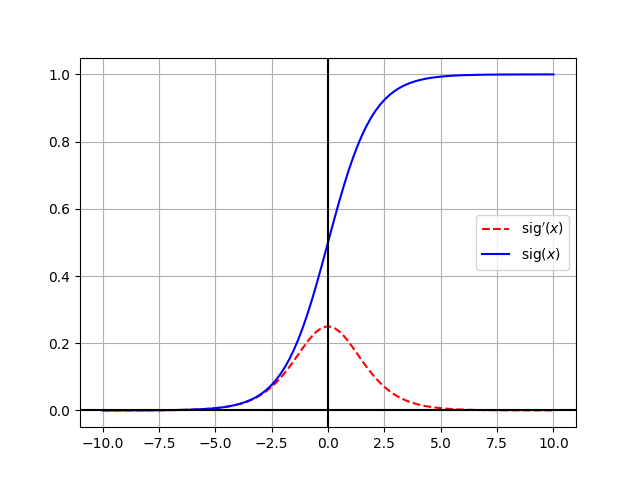
\includegraphics[width=\linewidth]{figures/neural_networks/activation_grads.png}
    \caption[]{Sigmoid activation gradients. Note that for \(\abs{x} > 5\) the gradient is almost 0.}\label{fig:activs}
\end{figure}
\begin{figure*}[!tb]
    \centering
    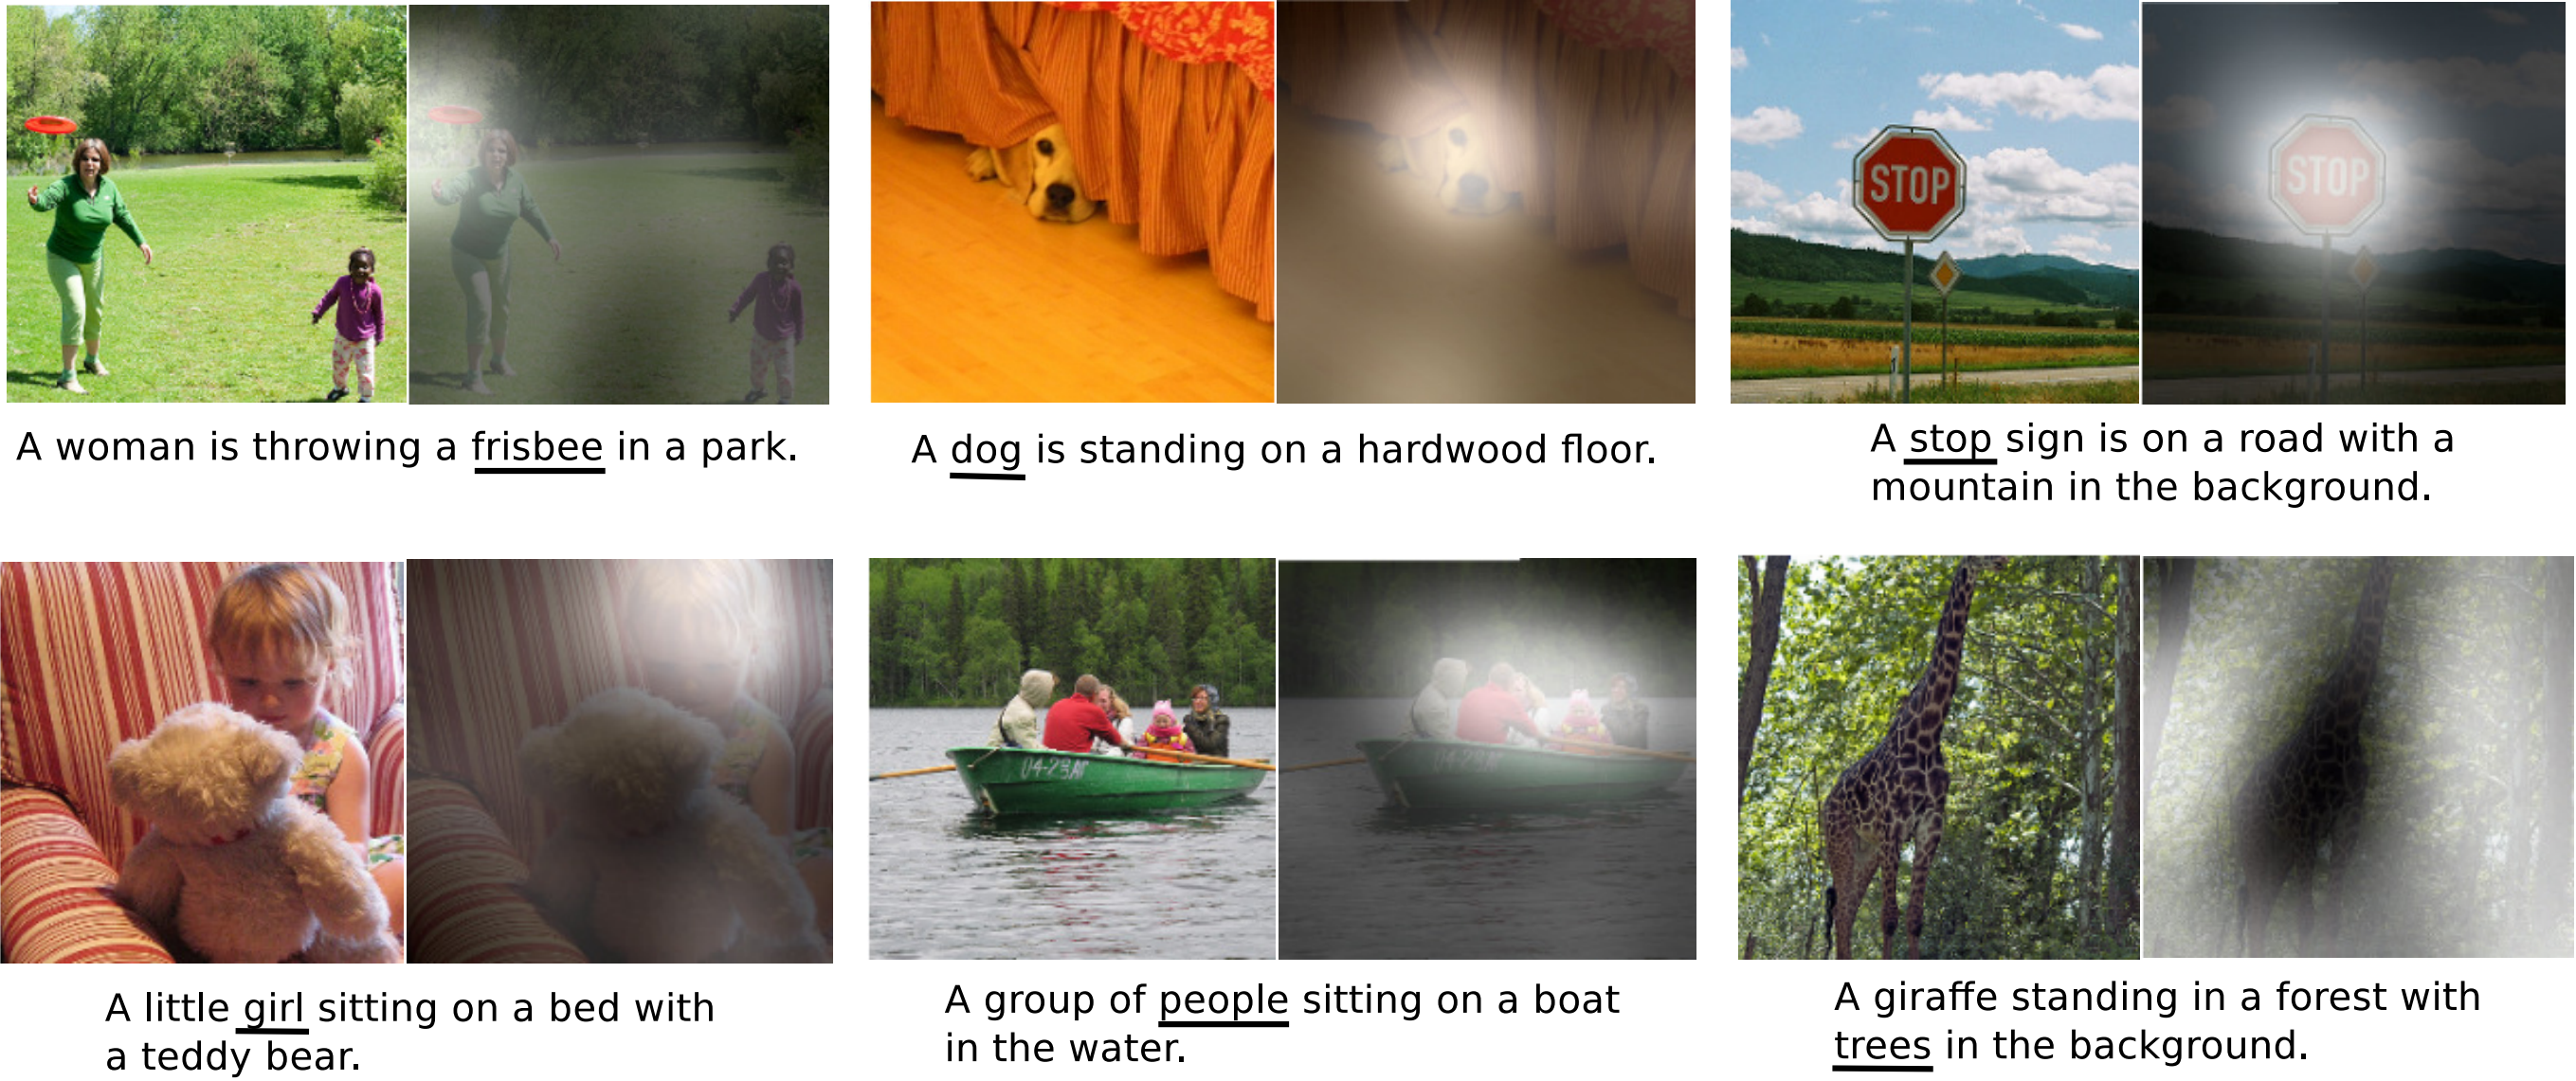
\includegraphics[width=\textwidth]{figures/neural_networks/attention.png}
    \caption[]{Attention for image captioning \cite{xu2015attend}.}\label{fig:attention}
\end{figure*}
\begin{figure}[!tb]
    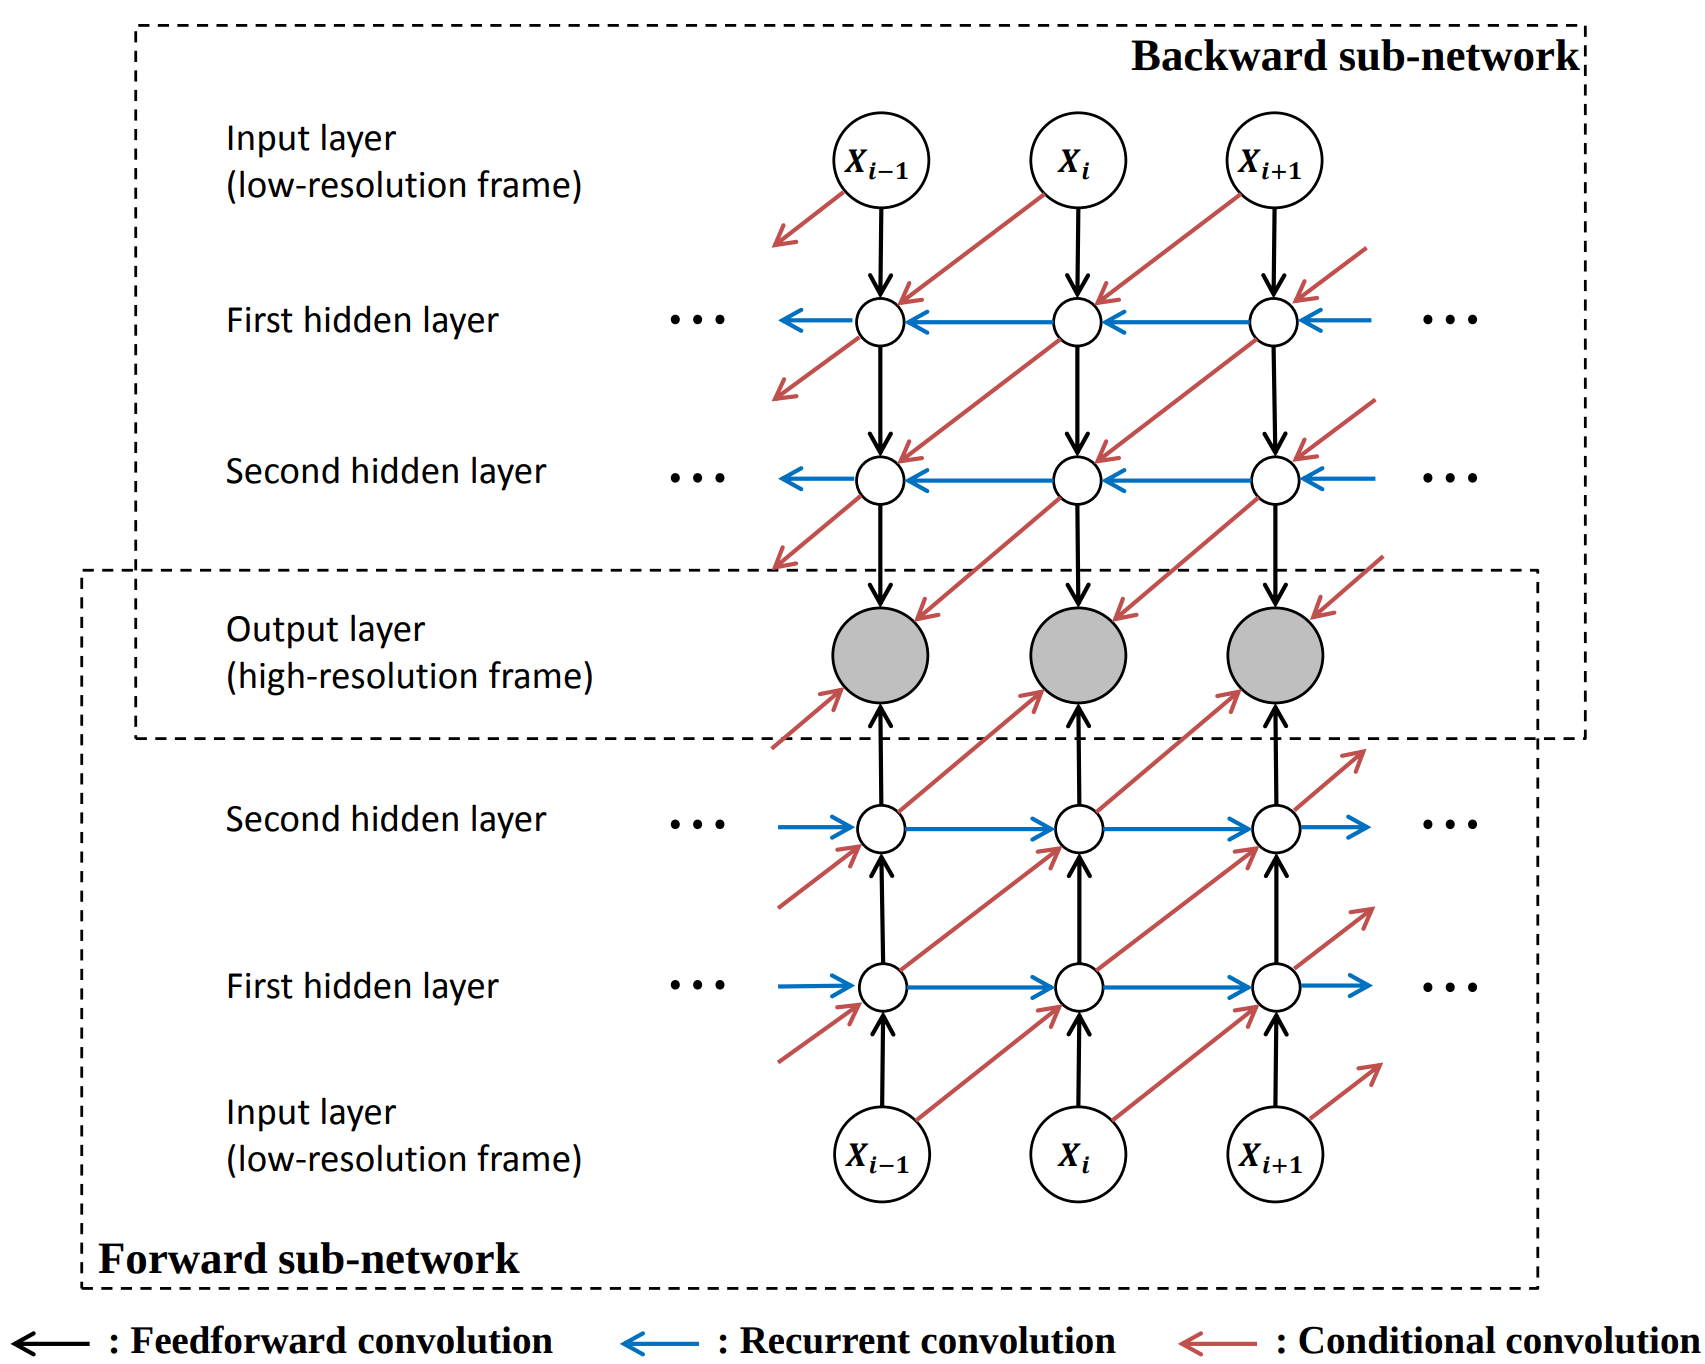
\includegraphics[width=.49\textwidth]{figures/neural_networks/brcn.png}
    \caption{BRCN schematic diagram \cite{huang2015bidirectional}.}\label{subfig:brcn}
\end{figure}
\begin{figure}[!tb]
    \centering
    \begin{subfigure}[b]{.49\textwidth}
        \centering
        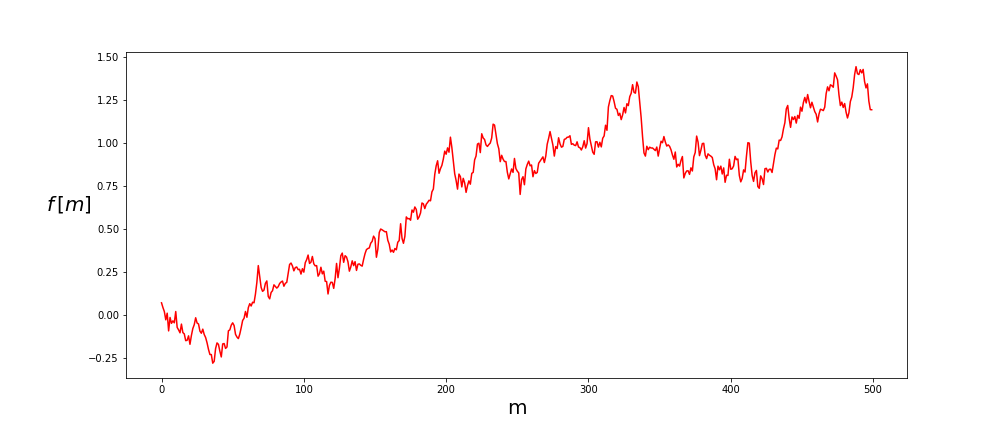
\includegraphics[width=0.95\textwidth]{figures/neural_networks/unsmoothed.png}
        \caption{Noisy function \(f\) (Wiener process sample).}\label{fig:convnoisy}
    \end{subfigure}

    \begin{subfigure}[b]{.49\textwidth}
        \centering
        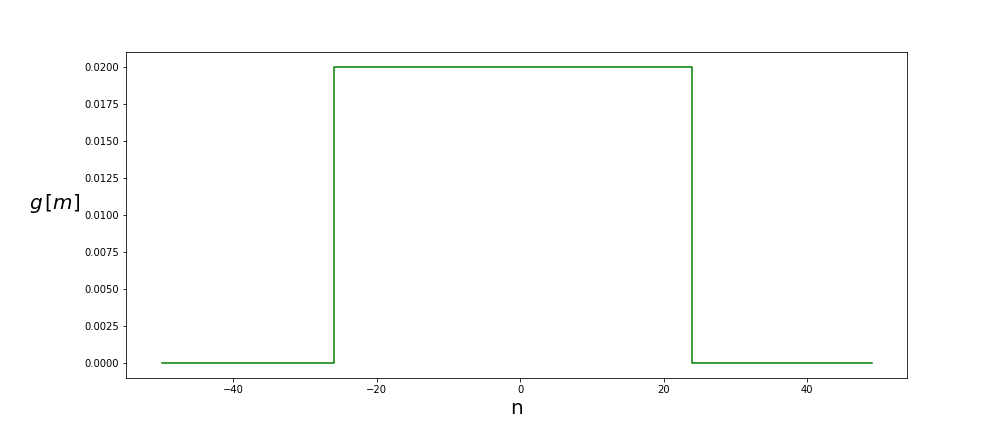
\includegraphics[width=0.95\textwidth]{figures/neural_networks/kernel.png}
        \caption{Heaviside function (low-pass filter \(g\)).}\label{fig:convfilter}
    \end{subfigure}
    \begin{subfigure}[b]{.49\textwidth}
        \centering
        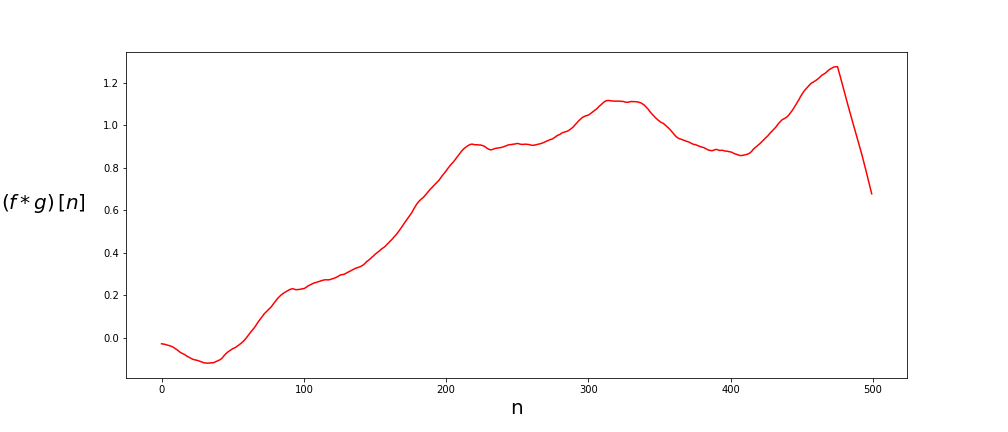
\includegraphics[width=0.95\textwidth]{figures/neural_networks/smoothed.png}
        \caption{Smoothed (low-pass filtered) \(f * g\).}\label{fig:convsmooth}
    \end{subfigure}
    \caption{Convolution as filtering.}\label{fig:convfiltering}
\end{figure}
\begin{figure*}[!tb]
    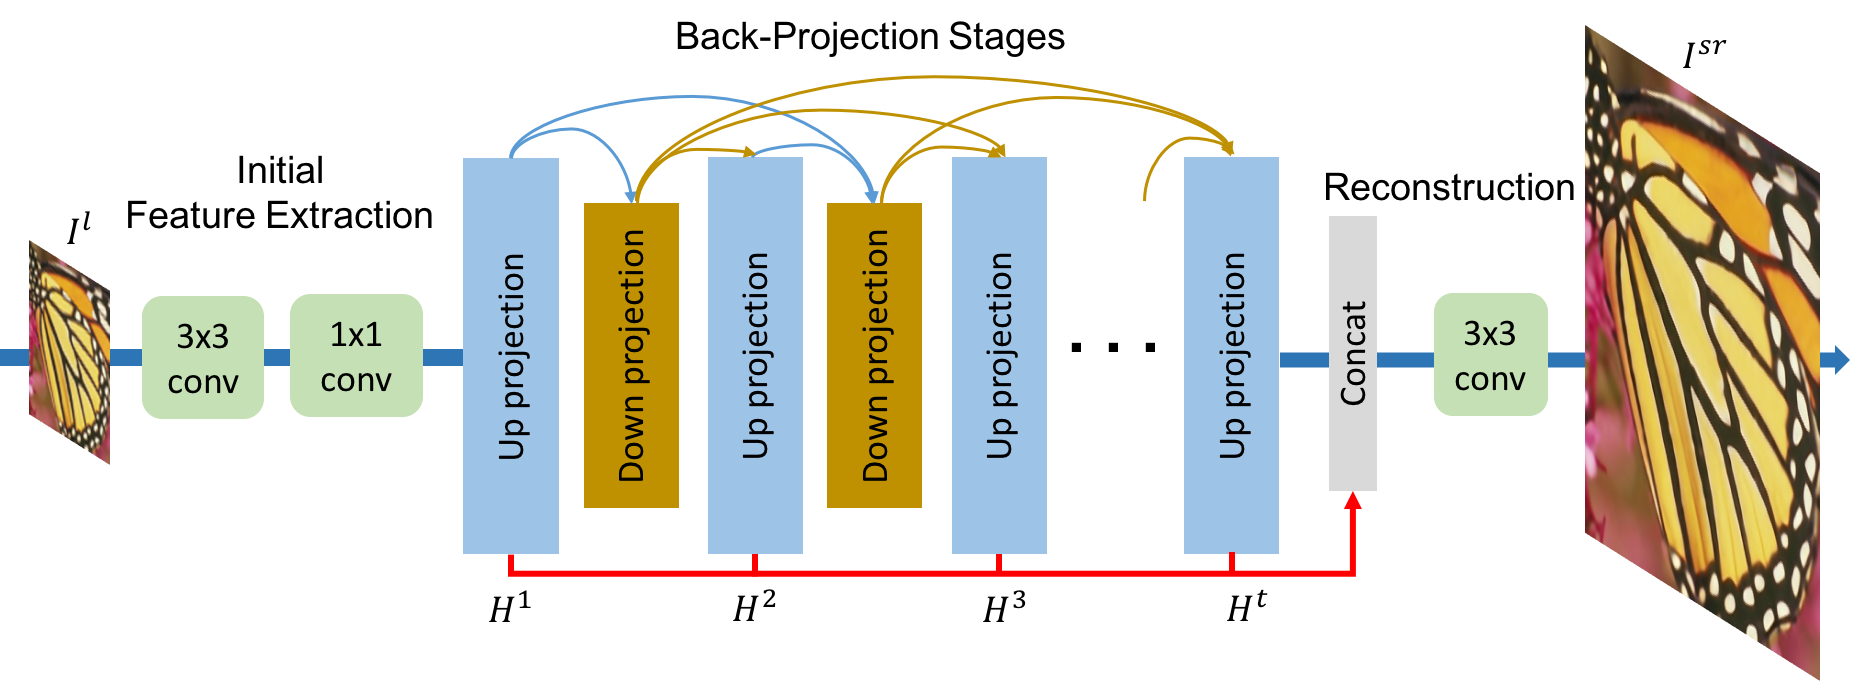
\includegraphics[width=\textwidth,keepaspectratio]{figures/neural_networks/DBPN.png}
    \caption{End-to-end DBPN network.}\label{fig:dbpn}
\end{figure*}
\begin{figure}[!tb]
    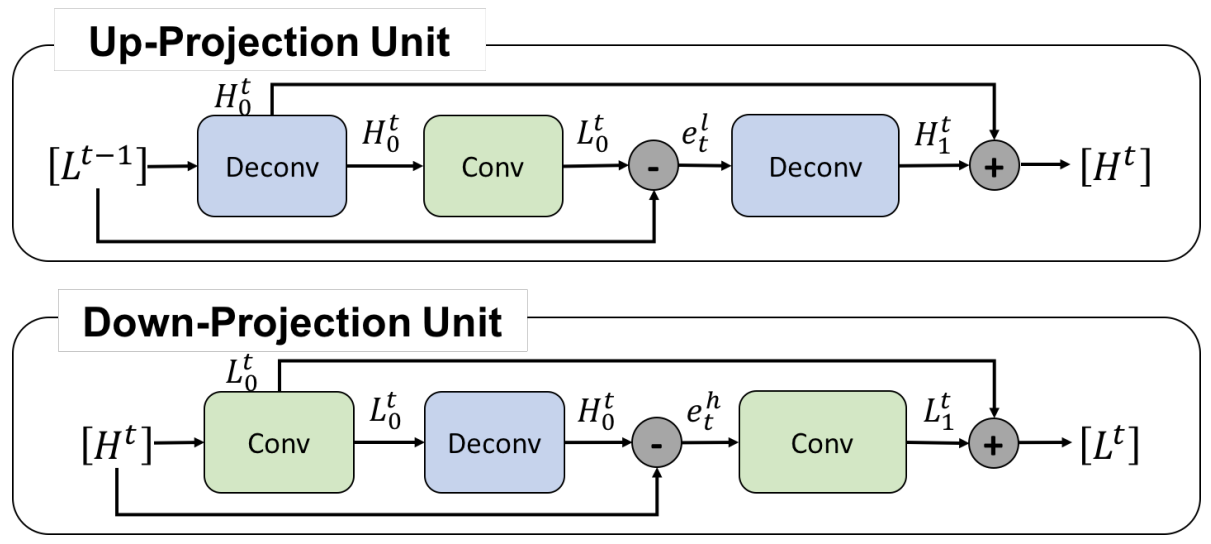
\includegraphics[width=.49\textwidth,keepaspectratio]{figures/neural_networks/up_down_up.png}
    \caption{DBPN Up, Down projection unit components implementing error correction.}\label{fig:updowndbpn}
\end{figure}
\begin{figure*}[!tb]
    \centering
    \begin{subfigure}[b]{0.33\textwidth}
        \centering
        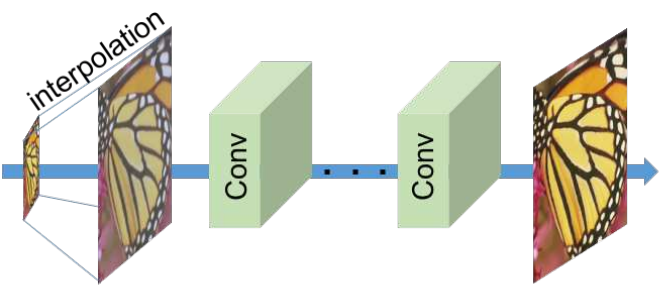
\includegraphics[width=0.95\textwidth]{figures/neural_networks/predefined_upsample.png}
        \caption{Predefined up-sampling.}\label{fig:predefups}
    \end{subfigure}
    \begin{subfigure}[b]{0.66\textwidth}
        \centering
        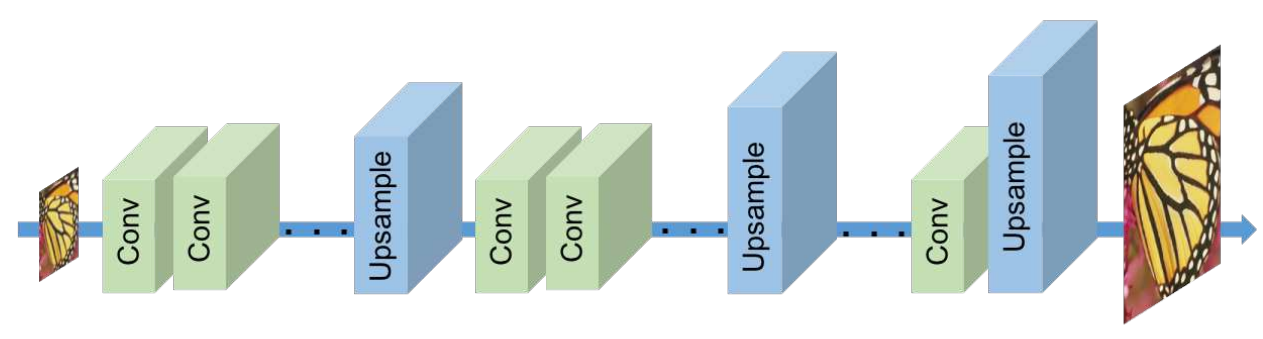
\includegraphics[width=0.95\textwidth]{figures/neural_networks/progressive_upsample.png}
        \caption{Progressive up-sampling.}\label{fig:profups}
    \end{subfigure}

    \begin{subfigure}[b]{0.33\textwidth}
        \centering
        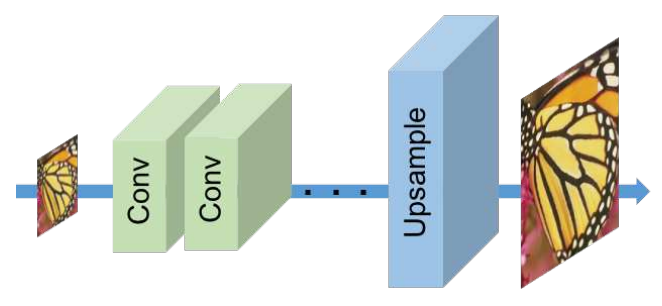
\includegraphics[width=0.95\textwidth]{figures/neural_networks/single_upsample.png}
        \caption{Single up-sampling.}\label{fig:singups}
    \end{subfigure}
    \begin{subfigure}[b]{0.66\textwidth}
        \centering
        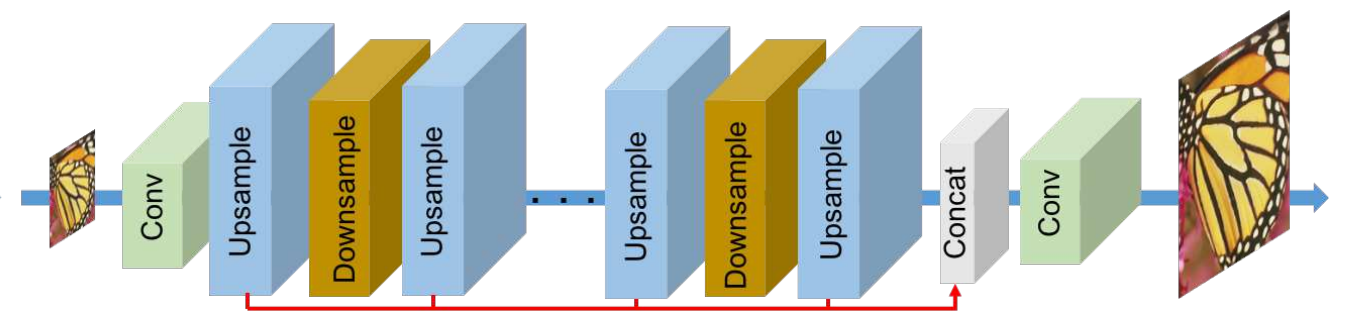
\includegraphics[width=0.95\textwidth]{figures/neural_networks/iterative_upsample.png}
        \caption{Iterative up-down-up-sampling.}\label{fig:iterups}
    \end{subfigure}
    \caption{Comparison of Deep SR network architectures \cite{haris2018deep}}\label{fig:comparedeepsr}
\end{figure*}
\begin{figure}[!tb]
    \centering
    \begin{subfigure}[b]{.49\textwidth}
        \centering
        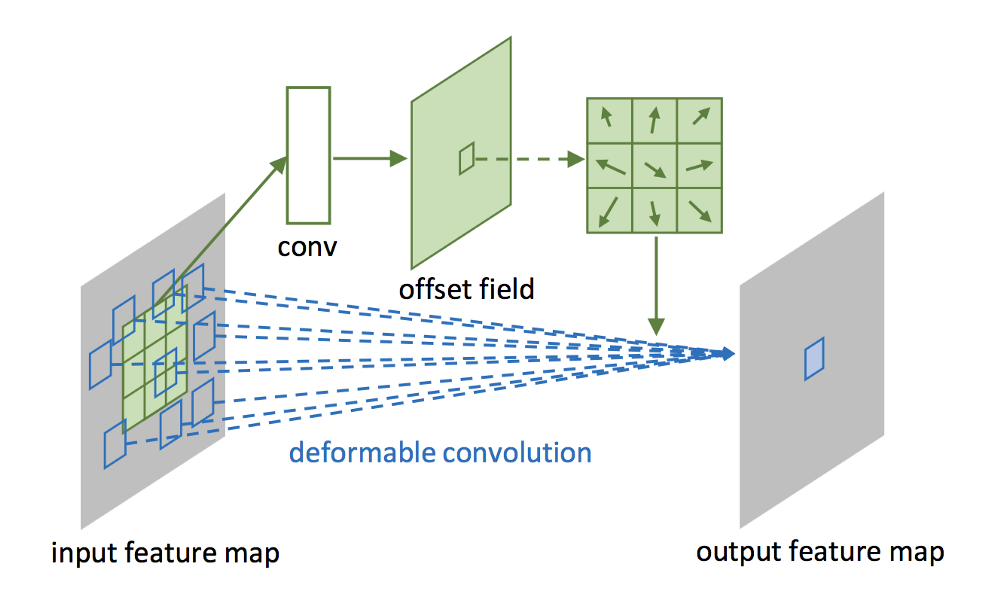
\includegraphics[width=\textwidth]{figures/neural_networks/deformable_conv.png}
        \caption{Illustration of 3 \(\times\) 3 deformable convolution.}\label{subfig:deform_conv}
    \end{subfigure}
    \vskip\baselineskip
    \begin{subfigure}[b]{.49\textwidth}
        \centering
        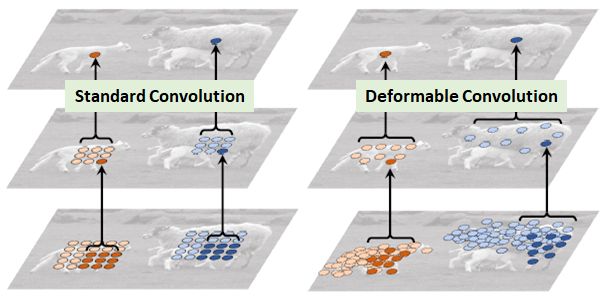
\includegraphics[width=\textwidth]{figures/neural_networks/standard_deformable_conv.png}
        \caption{Standard vs. deformable convolution.}\label{subfig:deform_conv}
    \end{subfigure}
    \caption[]{Deformable convolutions \cite{Dai_2017}.}\label{fig:deformconv}
\end{figure}
\begin{figure*}[!tb]
    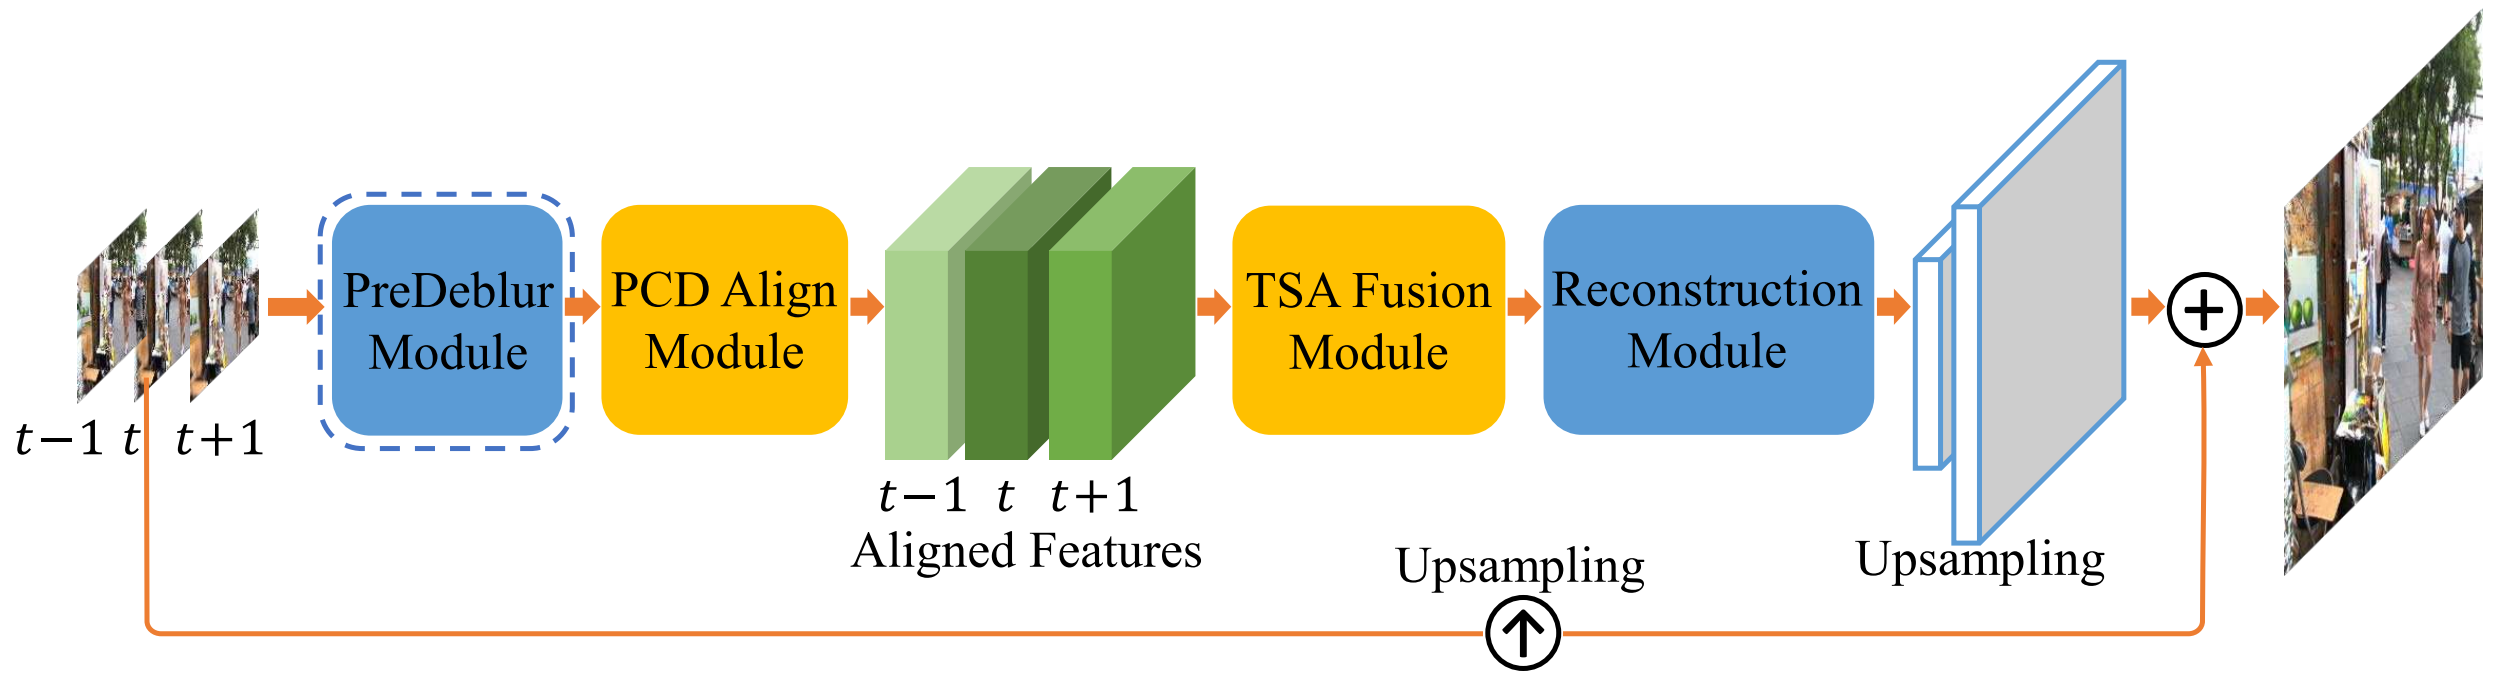
\includegraphics[width=\textwidth]{figures/neural_networks/edvr.png}
    \caption[]{Enhanced Deformable Convolutional Networks \cite{wang2019edvr}.}\label{fig:edvr}
\end{figure*}
\begin{figure*}[!tb]
    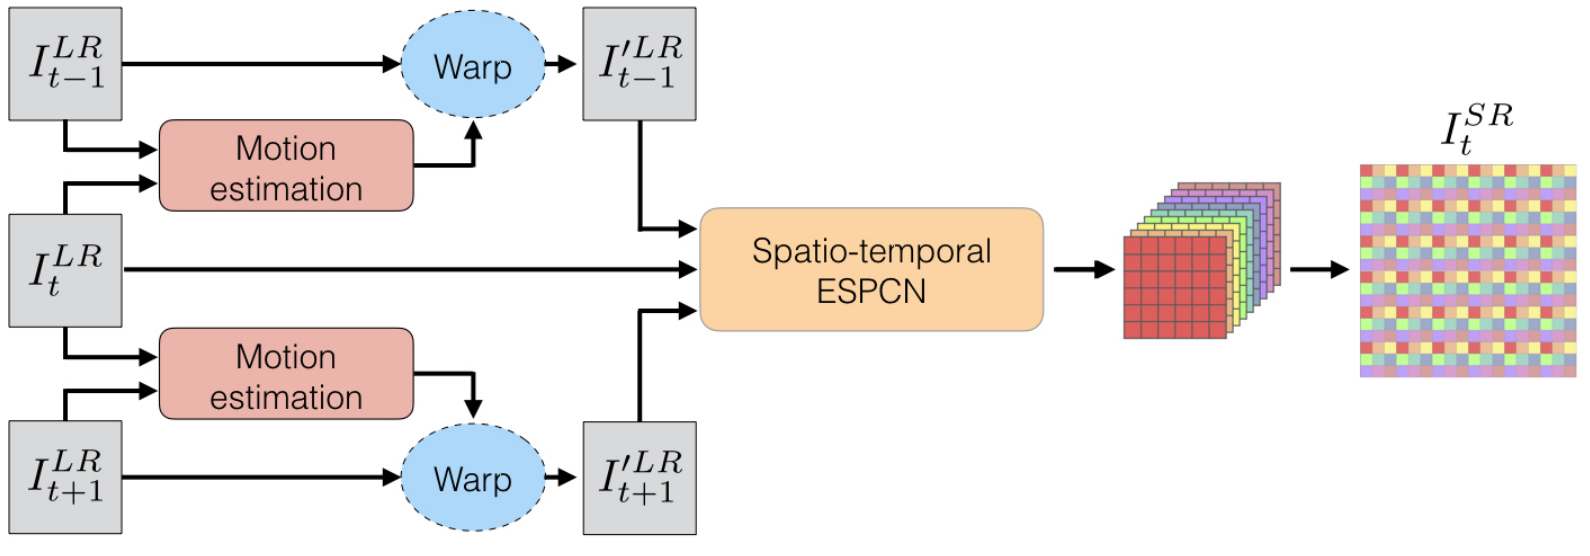
\includegraphics[width=\textwidth]{figures/neural_networks/realtime_epscn.png}
    \caption{Real-time MISR with motion compensation \cite{caballero2017real}. Motion compensation is performed two adjacent frames in a triplet and all three frames are then passed to up-sampling network.}\label{fig:realtimeepscn}
\end{figure*}
\begin{figure}[!tb]
    \centering
    \newcommand*{\subfigwidth}{0.49\textwidth}
    \begin{subfigure}[b]{\subfigwidth}
        \centering
        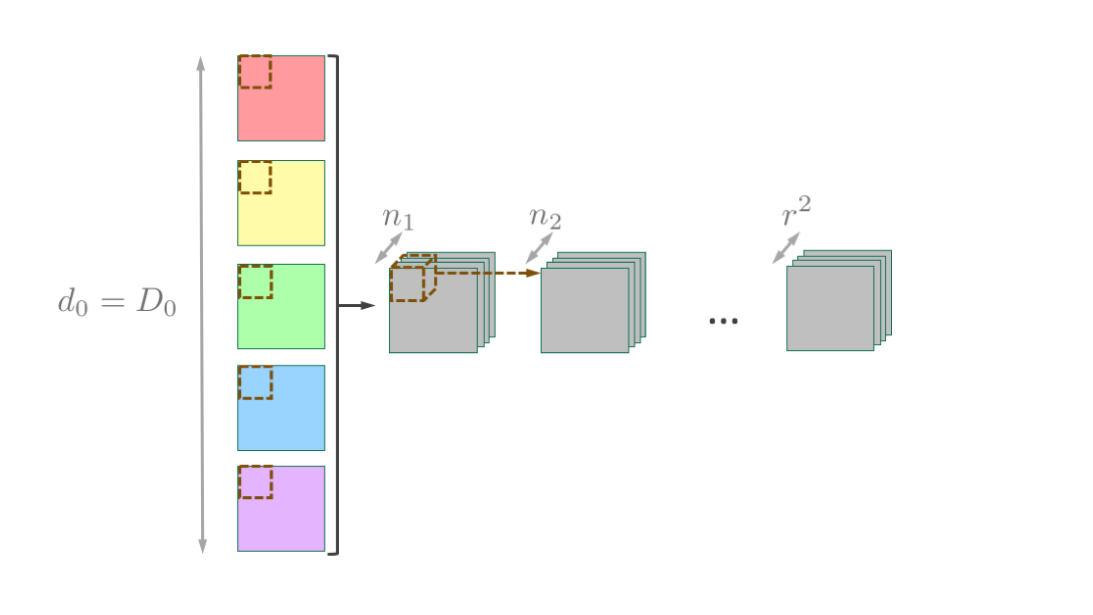
\includegraphics[width=.7\linewidth,keepaspectratio]{figures/neural_networks/early_fusion.png}
        \caption{Early fusion.}\label{subfig:earlyfus}
    \end{subfigure}
    \vskip\baselineskip
    \begin{subfigure}[b]{\subfigwidth}
        \centering
        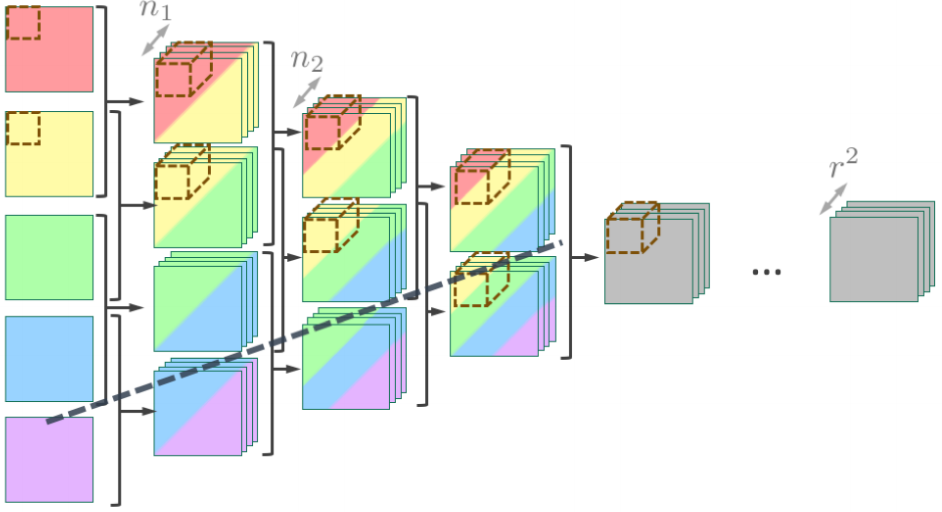
\includegraphics[width=\linewidth,keepaspectratio]{figures/neural_networks/slow_fusion.png}
        \caption{Slow fusion. If frames are processed in an online fashion then filter values should be shared. For example the last frame (purple) can recycle all of the computations above the dotted line.}\label{subfig:slowfus}
    \end{subfigure}
    % \vskip\baselineskip
    % \begin{subfigure}[b]{\subfigwidth}
    %     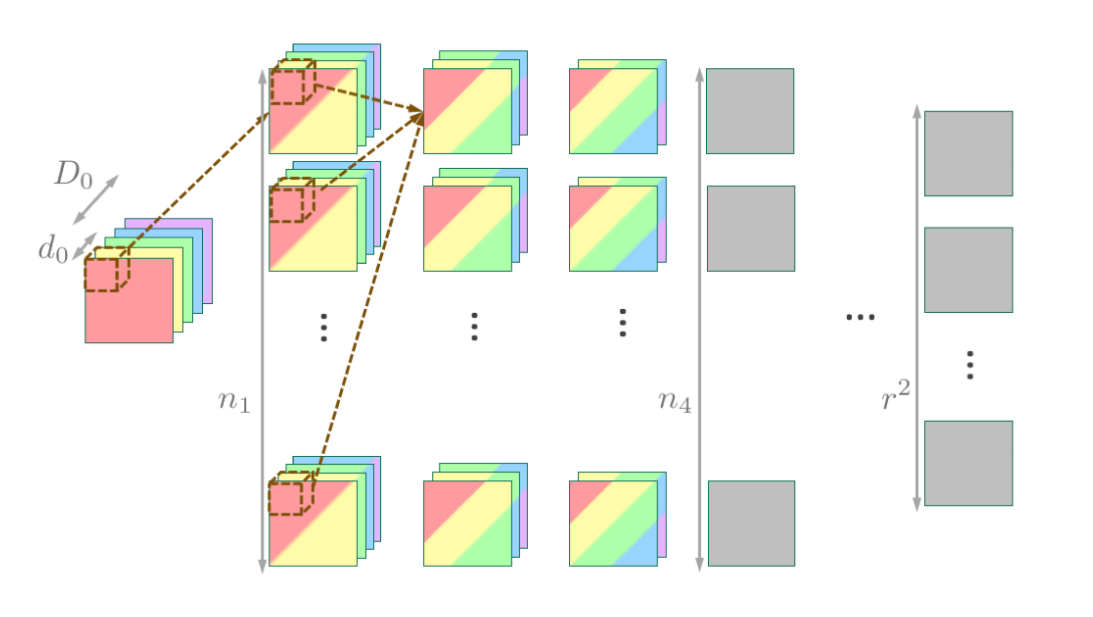
\includegraphics[width=\linewidth,keepaspectratio]{figures/neural_networks/3d_conv.png}
    %     \caption{3D convolution.}\label{subfig:updowndbpn}
    % \end{subfigure}
    \caption{Spatio-temporal ESPCN \cite{caballero2017real}.}\label{fig:fusions}
\end{figure}
\begin{figure}[!tb]
    \centering
    \begin{adjustbox}{width=\linewidth}
        \centering
        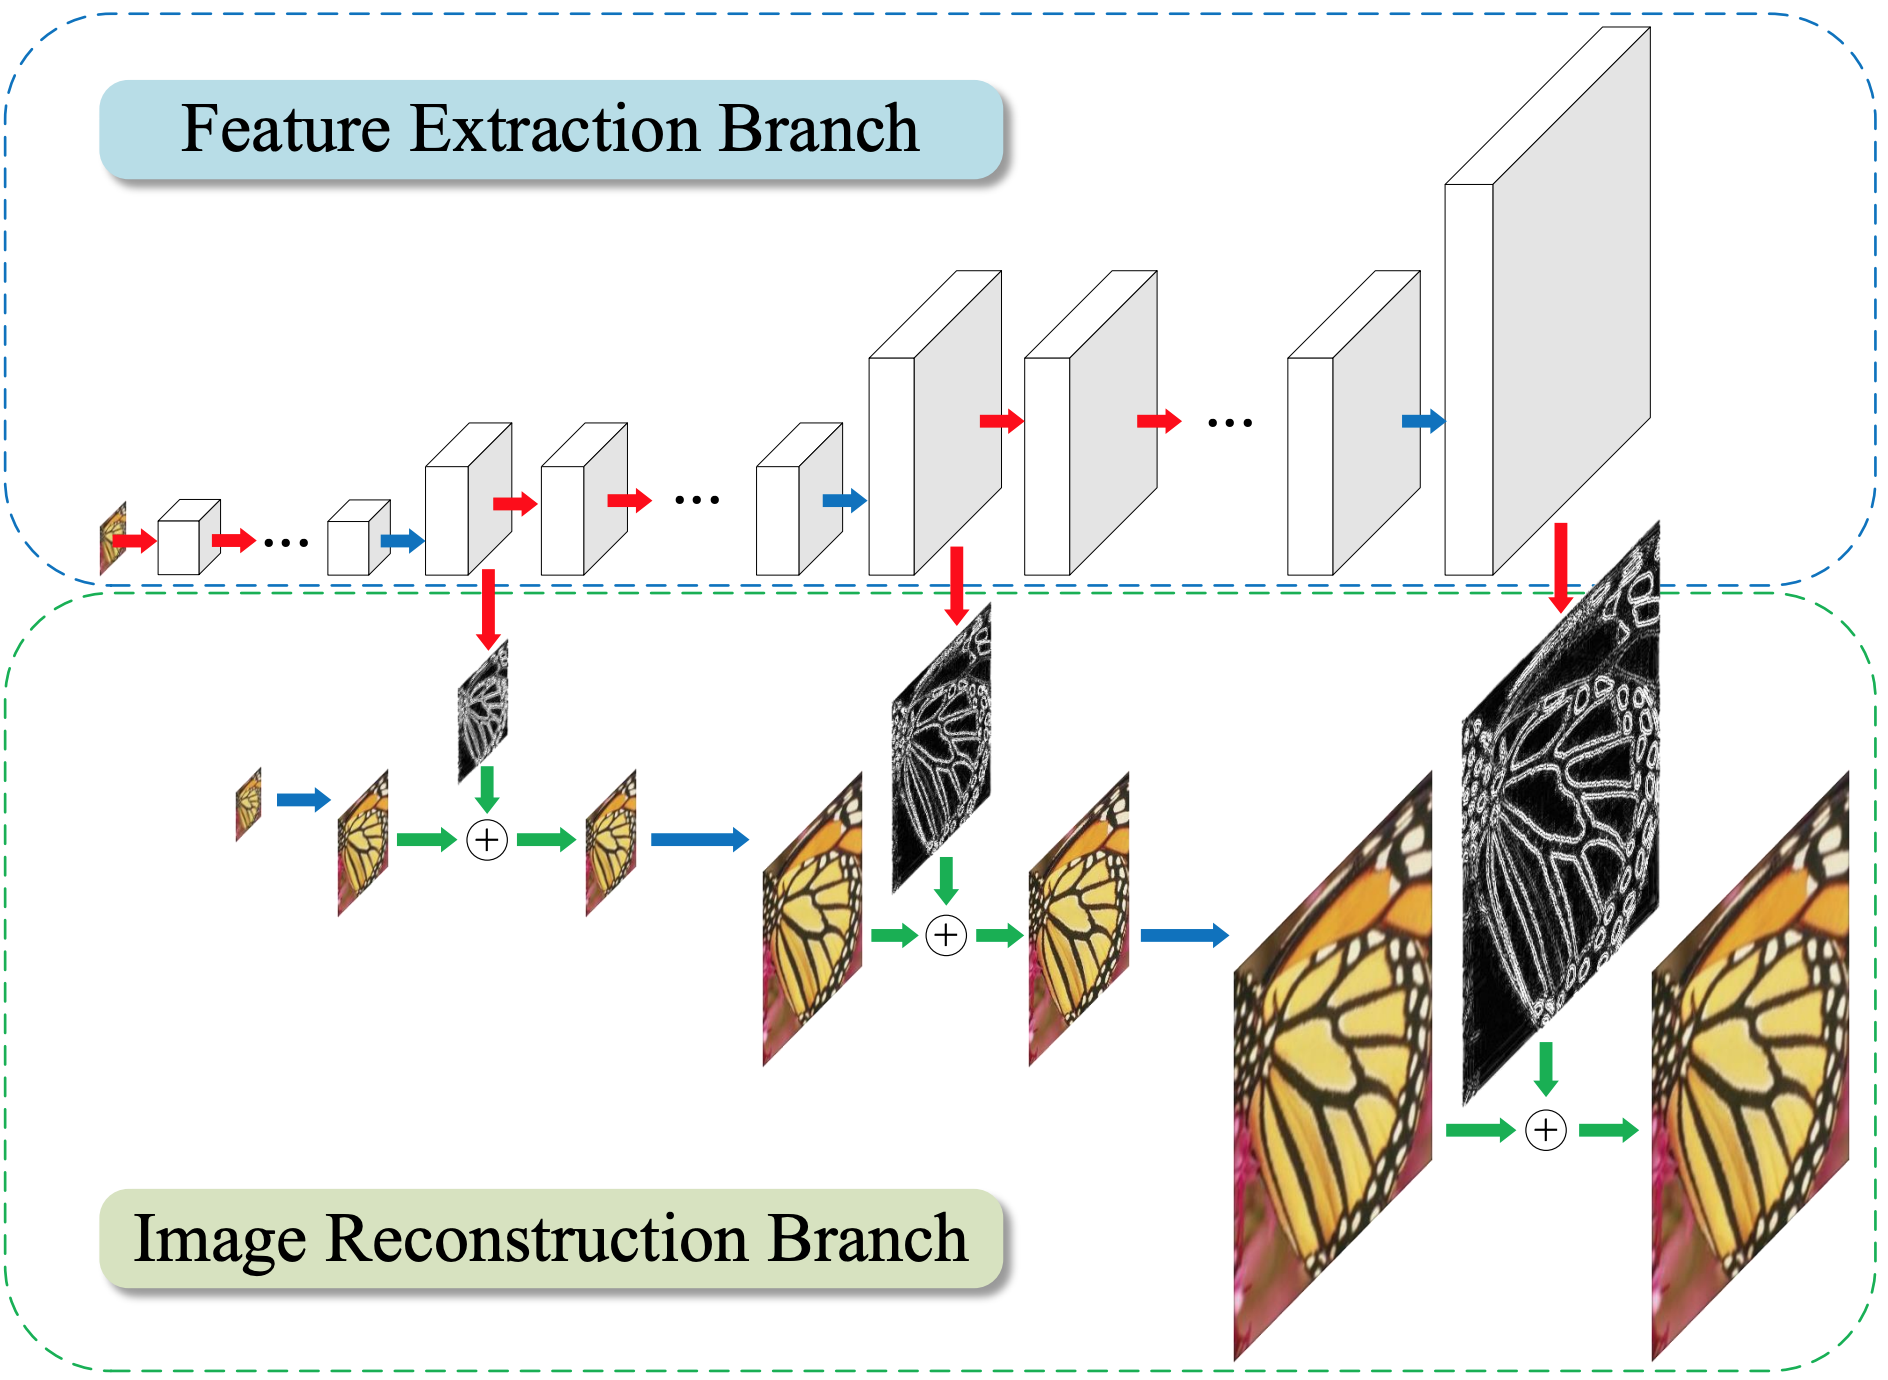
\includegraphics{figures/neural_networks/lapsrn.png}
    \end{adjustbox}
    \caption{LapSRN architecture \cite{Lai_2017}.}\label{fig:lapsrn}
\end{figure}
\begin{figure}[!tb]
    \centering
    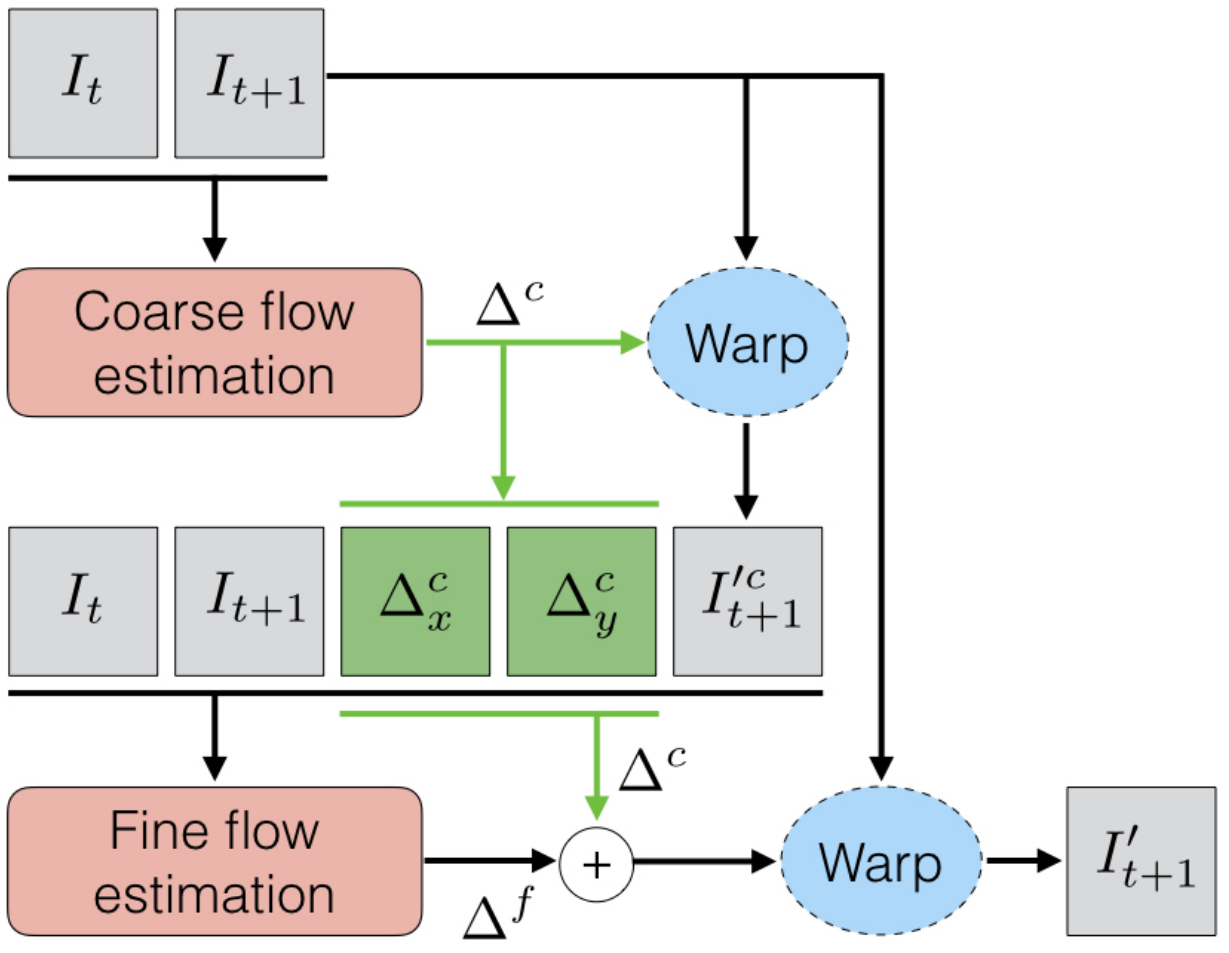
\includegraphics[width=.4\textwidth]{figures/neural_networks/motion_compensation.png}
    \caption{Motion estimation module for BRCN \cite{caballero2017real}.}\label{fig:motion_estimation}
\end{figure}
\begin{figure}[!tb]
    \centering
    \begin{adjustbox}{width=\linewidth}
        \centering
        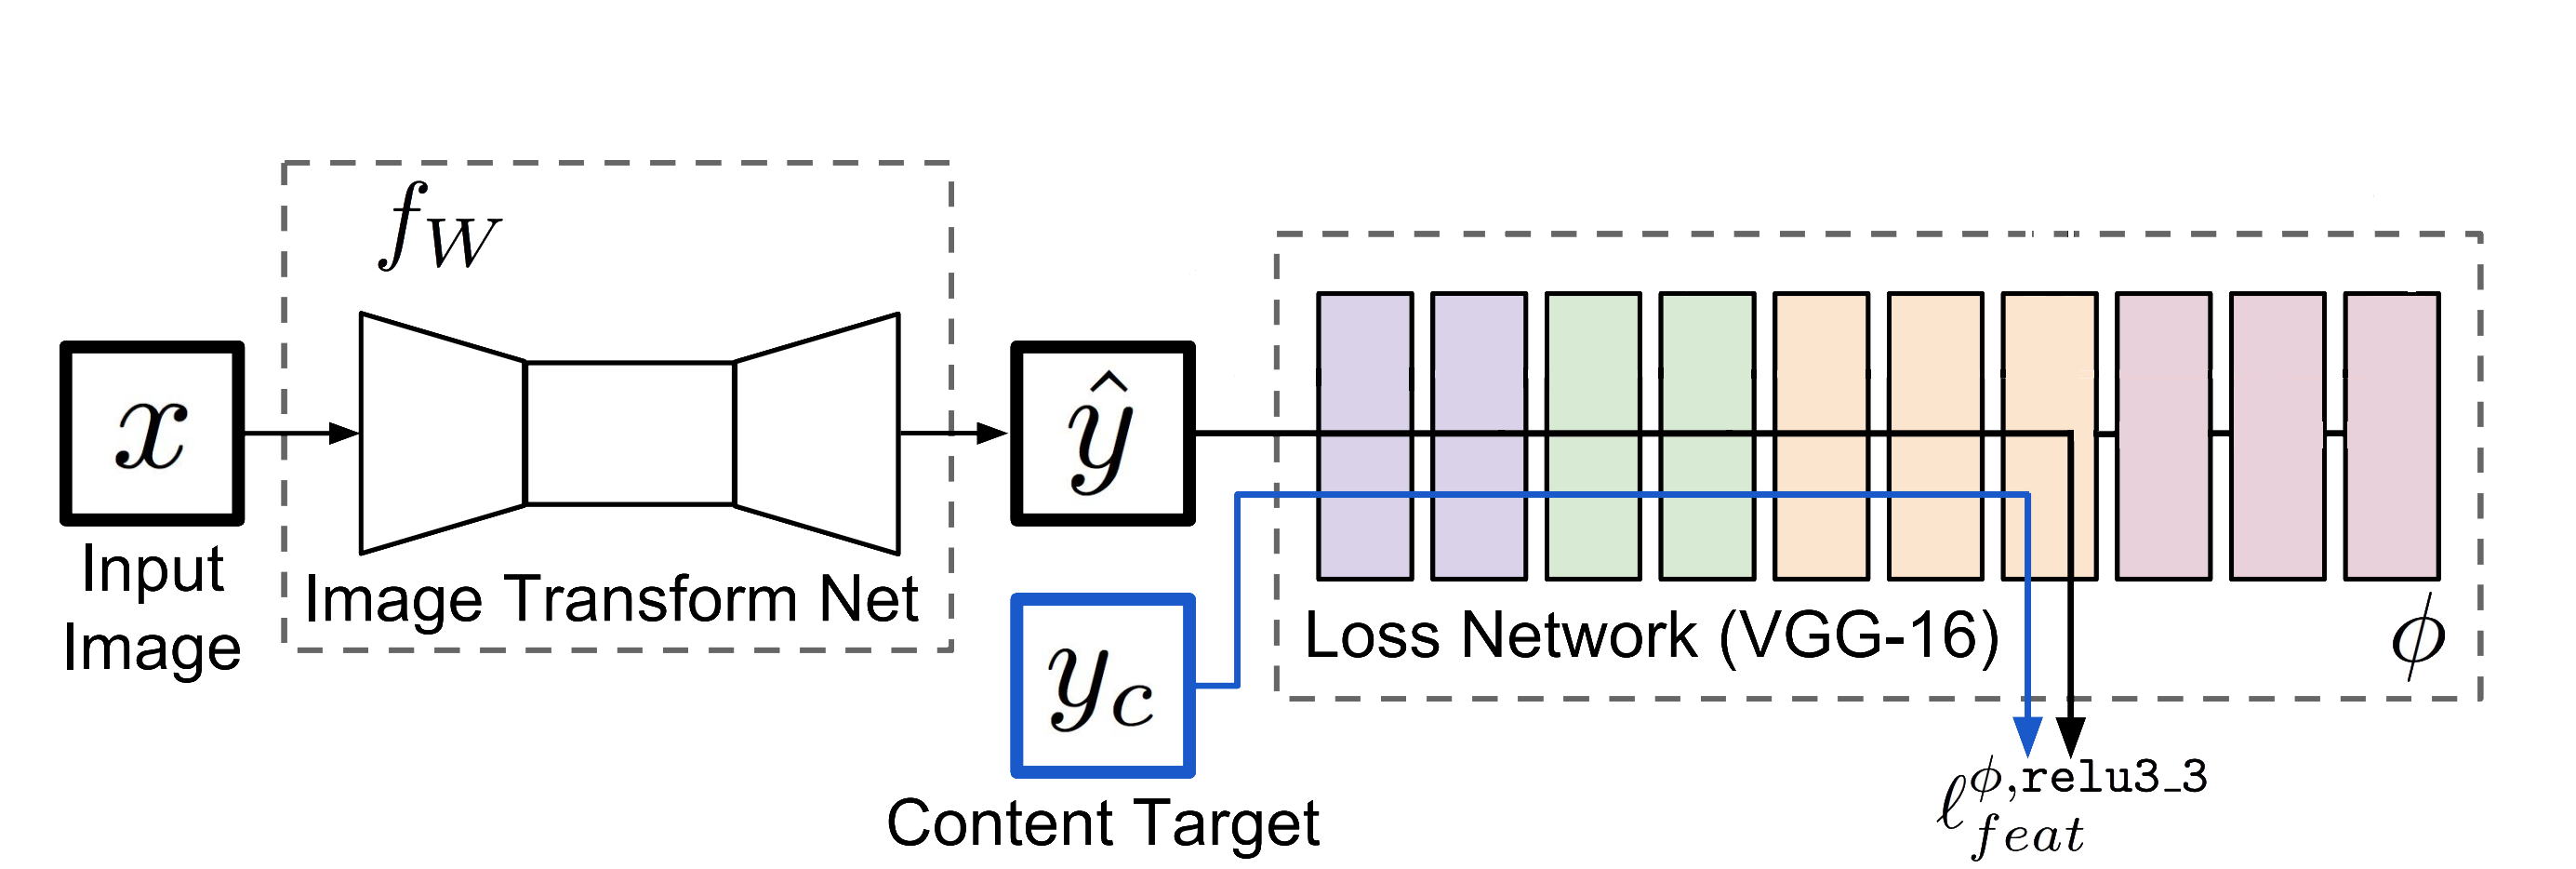
\includegraphics[]{figures/neural_networks/perceptual_loss.png}
    \end{adjustbox}
    \caption{Perceptual loss \cite{johnson2016perceptual}.}\label{fig:perceptualloss}
\end{figure}
\begin{figure*}[!tb]
    \centering
    \begin{subfigure}[b]{.39\textwidth}
        \centering
        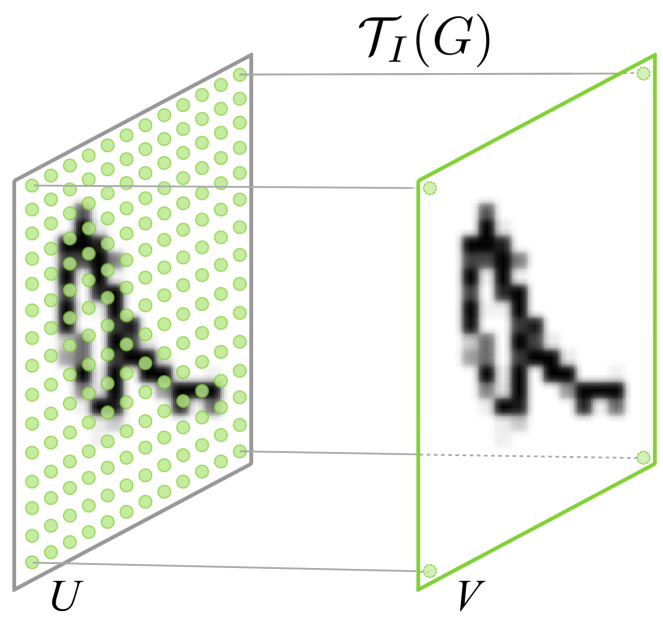
\includegraphics[width=\textwidth]{figures/neural_networks/space_transformer_ti.png}
        \caption{Sampling grid \(G' = \mathcal{T}_I(G)\) where \(I\) is the identity transformation.}\label{subfig:spacetransformer_ti}
    \end{subfigure}
    \hspace{35pt}
    \begin{subfigure}[b]{.39\textwidth}
        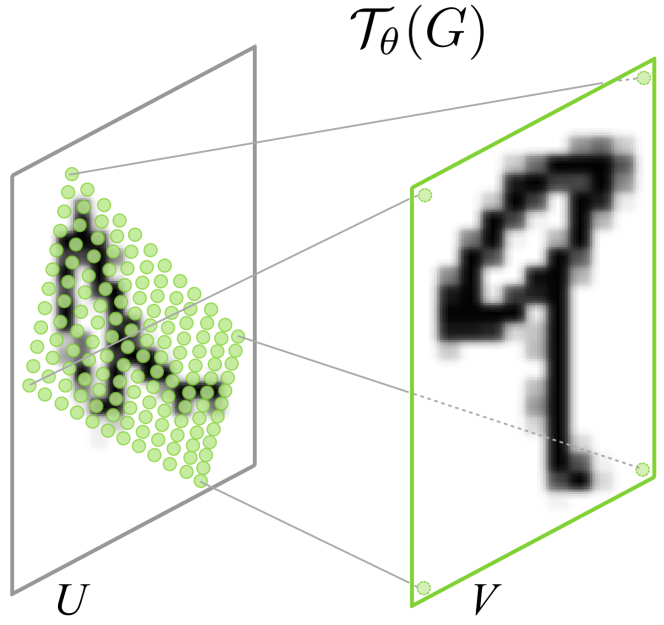
\includegraphics[width=\textwidth]{figures/neural_networks/space_transformer_ttheta.png}
        \caption{Sampling grid \(G' = \mathcal{T}_{\bm{\theta}}(G)\) where \(\bm{\theta}\) defines a 2D affine transformation.}\label{subfig:spacetransformer_ttheta}
    \end{subfigure}
    \caption{Parameterised sampling of image \(U\) to produce image \(V\) \cite{jaderberg2015spatial}.}\label{fig:paramsampling}
\end{figure*}
\begin{figure}[!tb]
    \centering
    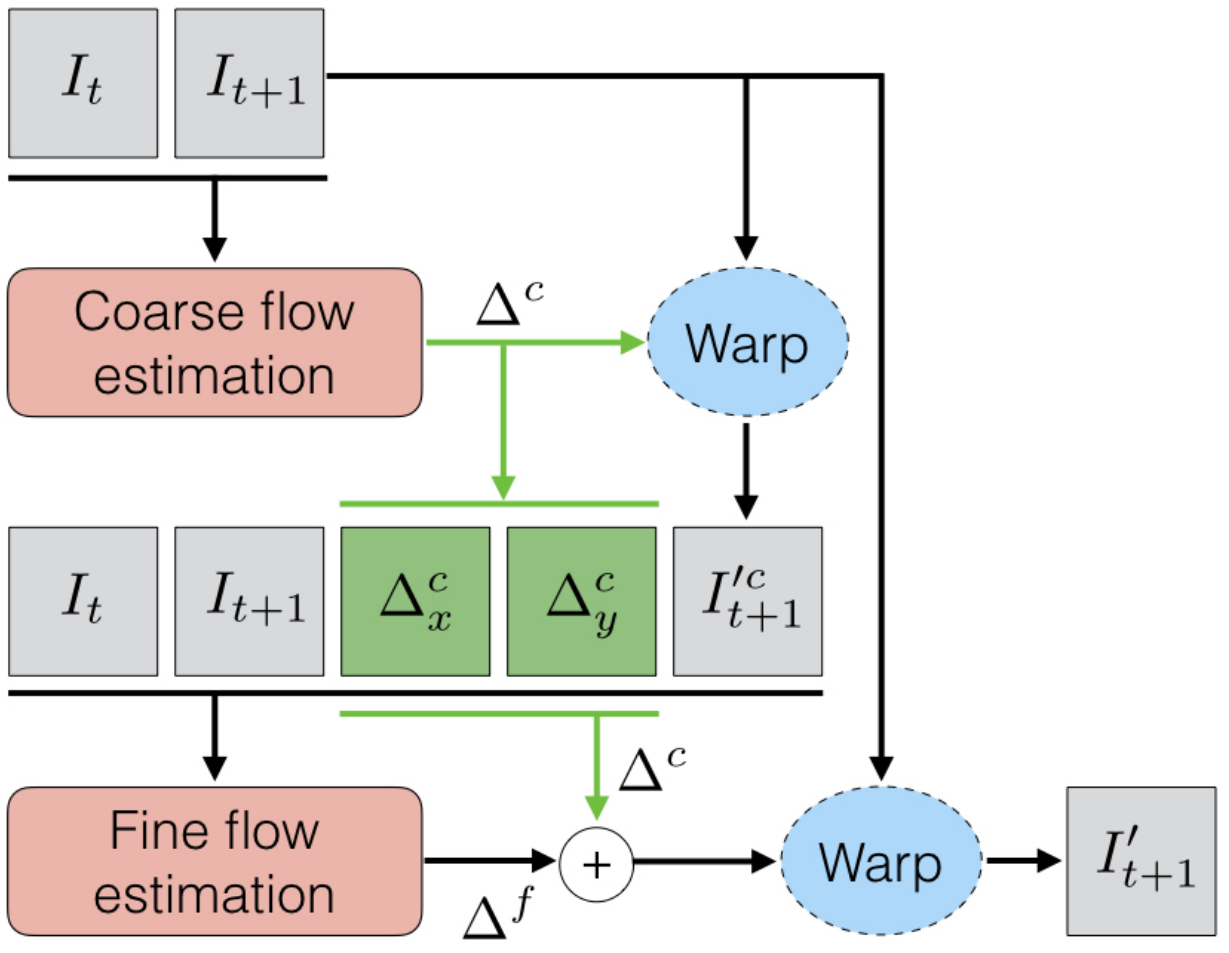
\includegraphics[width=.49\textwidth]{figures/neural_networks/space_transformer.png}
    \caption{Spatial Transformer \cite{jaderberg2015spatial}.}\label{fig:spacetransformer}
\end{figure}
\begin{figure}[!tb]
    \centering
    \newcommand*{\subfigwidth}{0.49\textwidth}
    \begin{subfigure}[b]{\subfigwidth}
        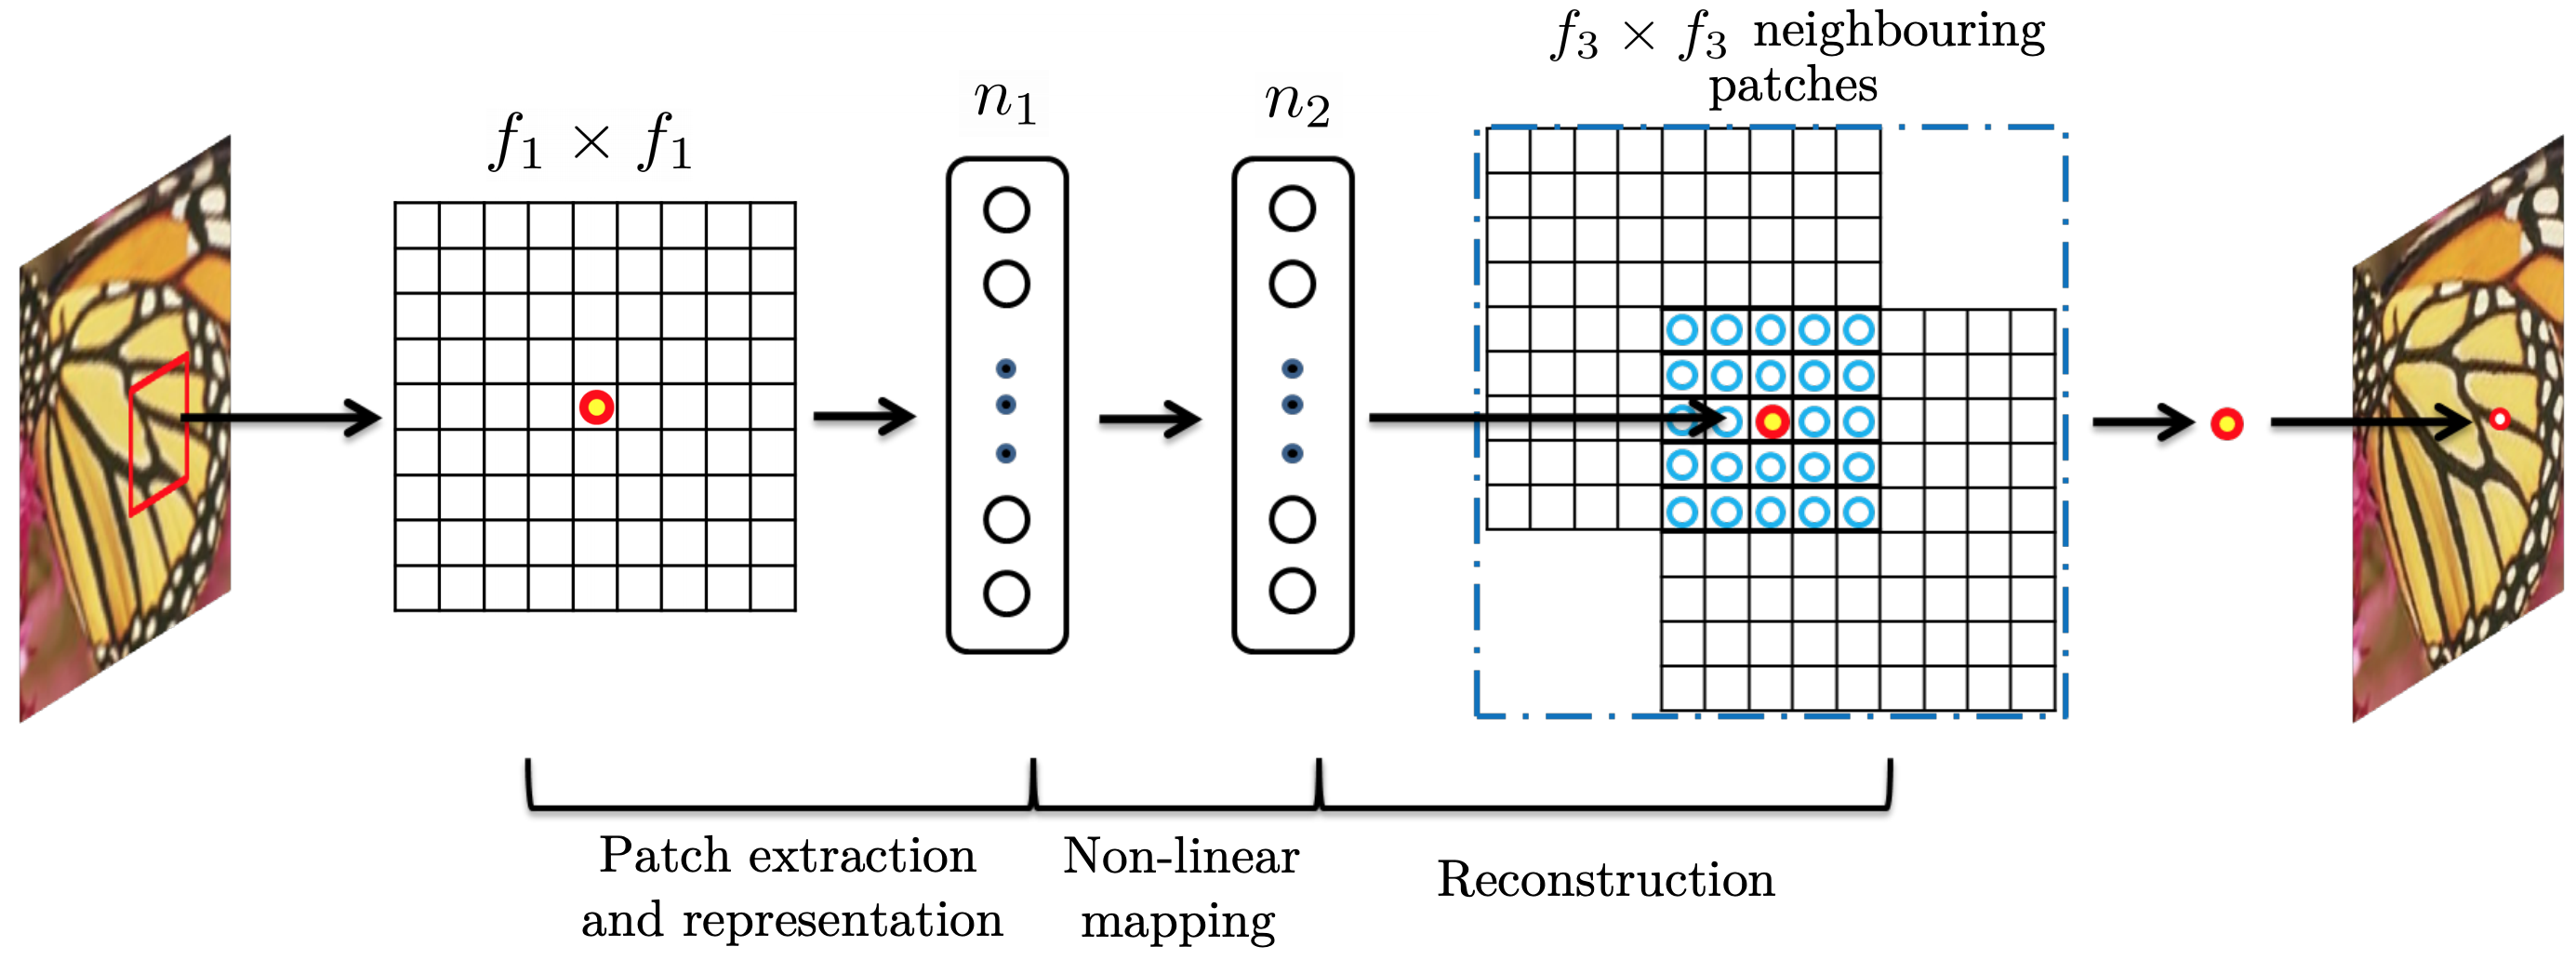
\includegraphics[width=\linewidth,keepaspectratio]{figures/neural_networks/sparse_coding.png}
        \caption{Sparse coding SR pipeline (see section~\ref{subsubsec:sparsecoding}).}\label{subfig:srcnnsparse}
    \end{subfigure}
    \vskip\baselineskip
    \begin{subfigure}[b]{\subfigwidth}
        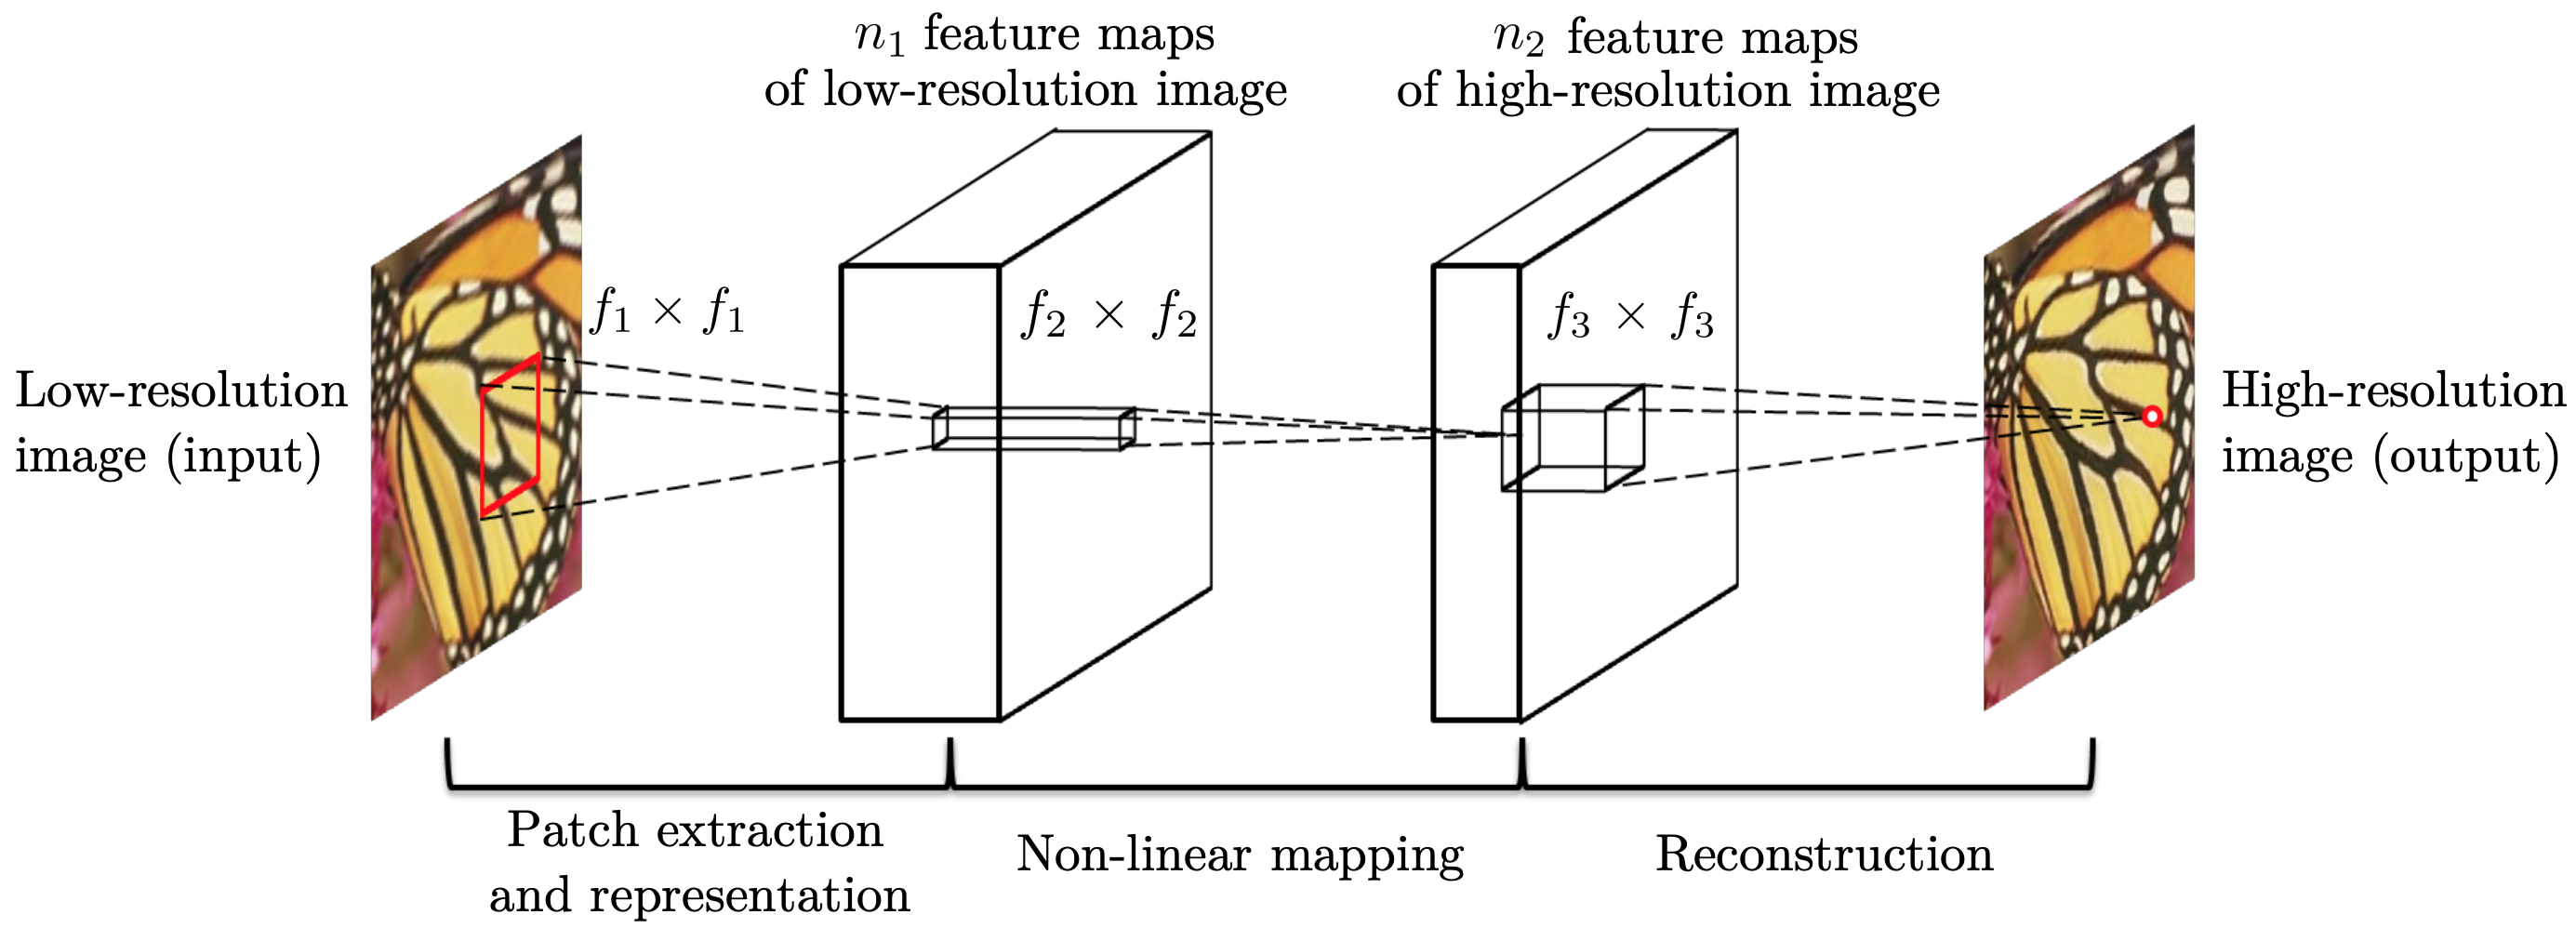
\includegraphics[width=\linewidth,keepaspectratio]{figures/neural_networks/srcnn.png}
        \caption{SRCNN pipeline.}\label{subfig:srcnn}
    \end{subfigure}
    \caption{Sparse coding SR and SRCNN comparison \cite{Dong_2016}. Note both pipelines operate on bicubic up-sampled images.}\label{fig:srcnn}
\end{figure}
\begin{figure}[!tb]
    \centering
    \begin{adjustbox}{width=\linewidth}
        \centering
        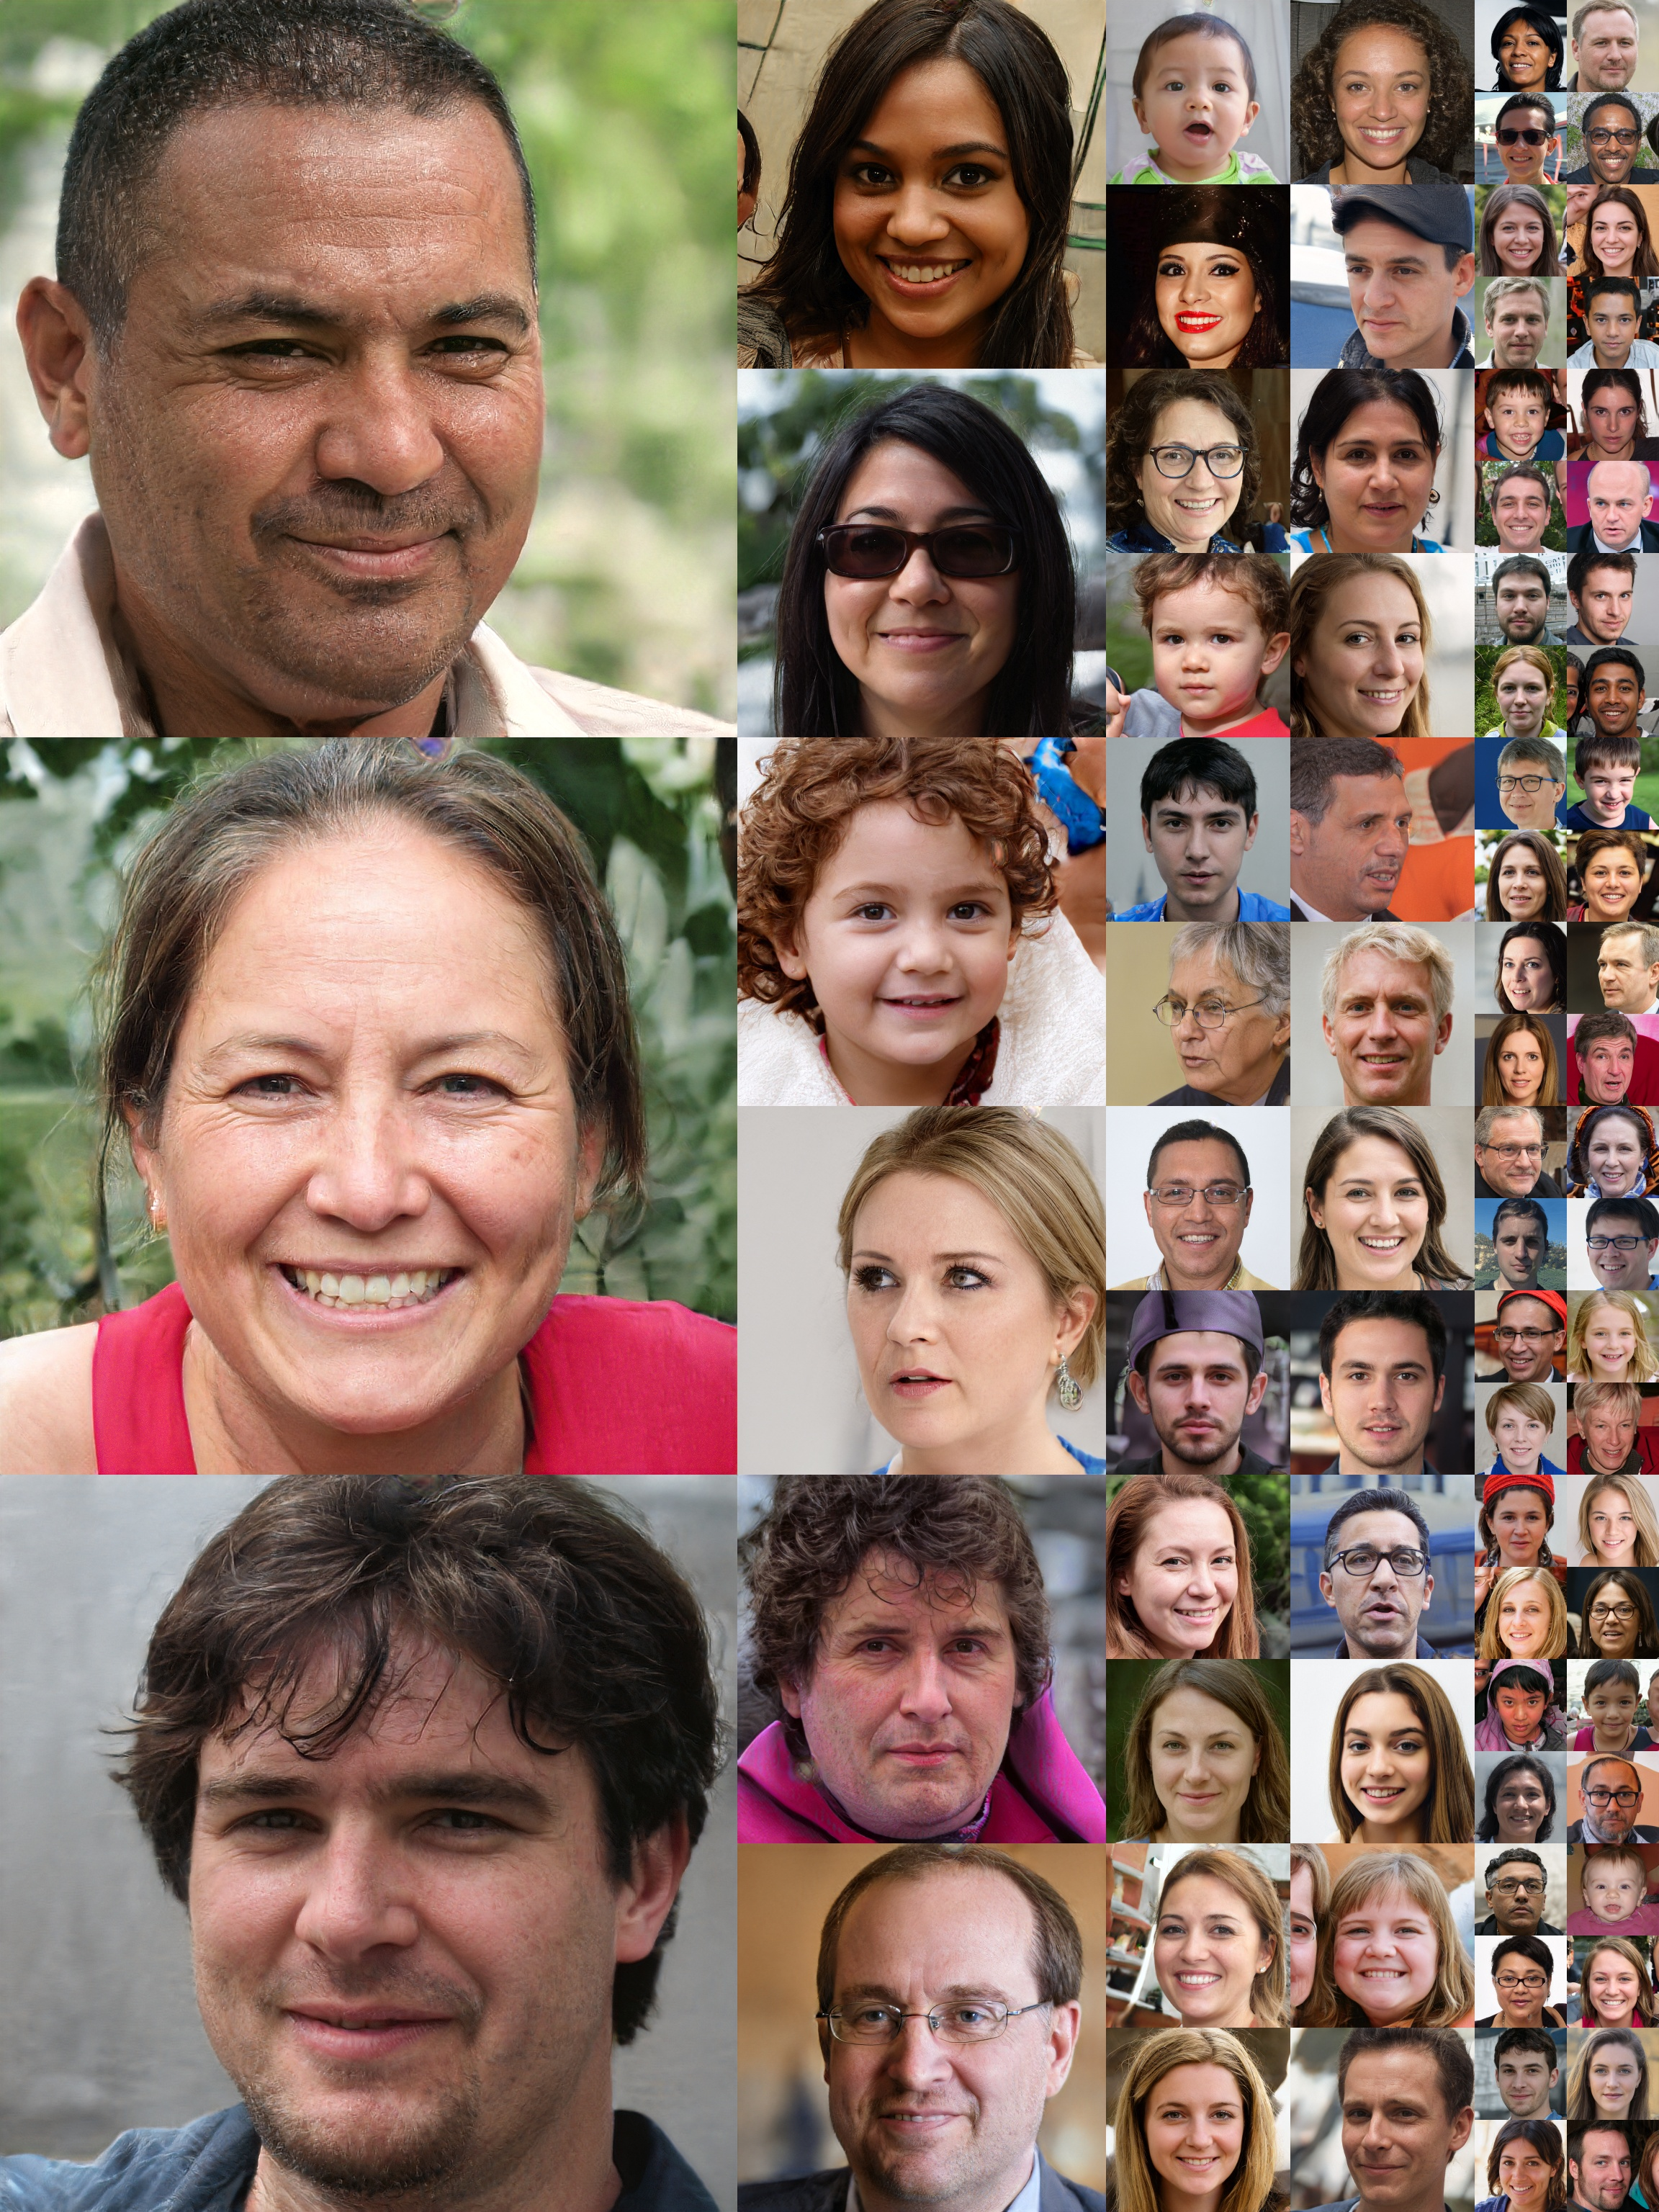
\includegraphics[]{figures/neural_networks/stylegan.jpg}
    \end{adjustbox}
    \caption{Uncurated set of images \textbf{generated} (i.e., none of the people depicted are real) using StyleGAN with the FFHQ dataset \cite{karras2018stylebased}.}\label{fig:stylegan}
\end{figure}
\begin{figure}[!tb]
    \centering
    \newcommand*{\subfigwidth}{.49\textwidth}
    \begin{subfigure}[b]{\subfigwidth}
        \centering
        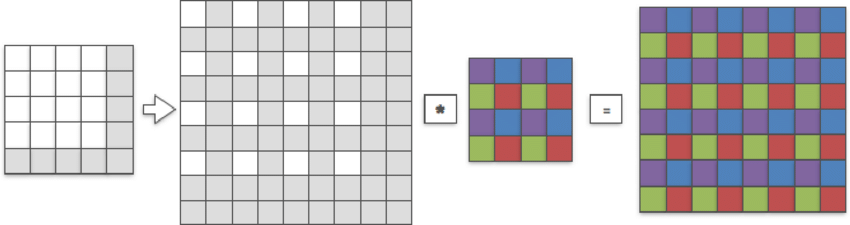
\includegraphics[width=\textwidth]{figures/neural_networks/subpixelconv1.png}
        \caption{Sub-pixel convolution as dilation then filtering.}\label{subfig:subpixdilate}
    \end{subfigure}
    \vskip\baselineskip
    \begin{subfigure}[b]{\subfigwidth}
        \centering
        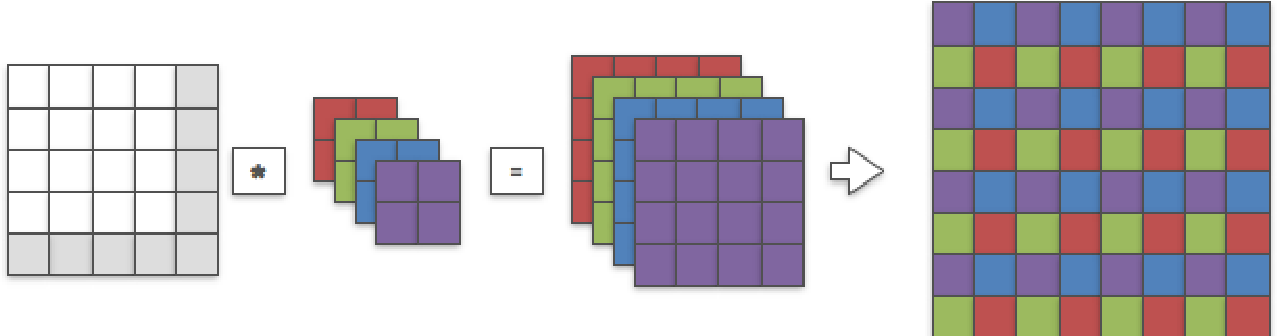
\includegraphics[width=\textwidth]{figures/neural_networks/subpixelconv2.png}
        \caption{Sub-pixel convolution as filtering then pixel-shuffling.}\label{subfig:pixelshuffle}
    \end{subfigure}
    \caption{Sub-pixel convolution.}\label{fig:subpixelconv}
\end{figure}
\begin{figure}[!tb]
    \centering
    \newcommand*{\subfigwidth}{0.49\textwidth}
    \begin{subfigure}[b]{\subfigwidth}
        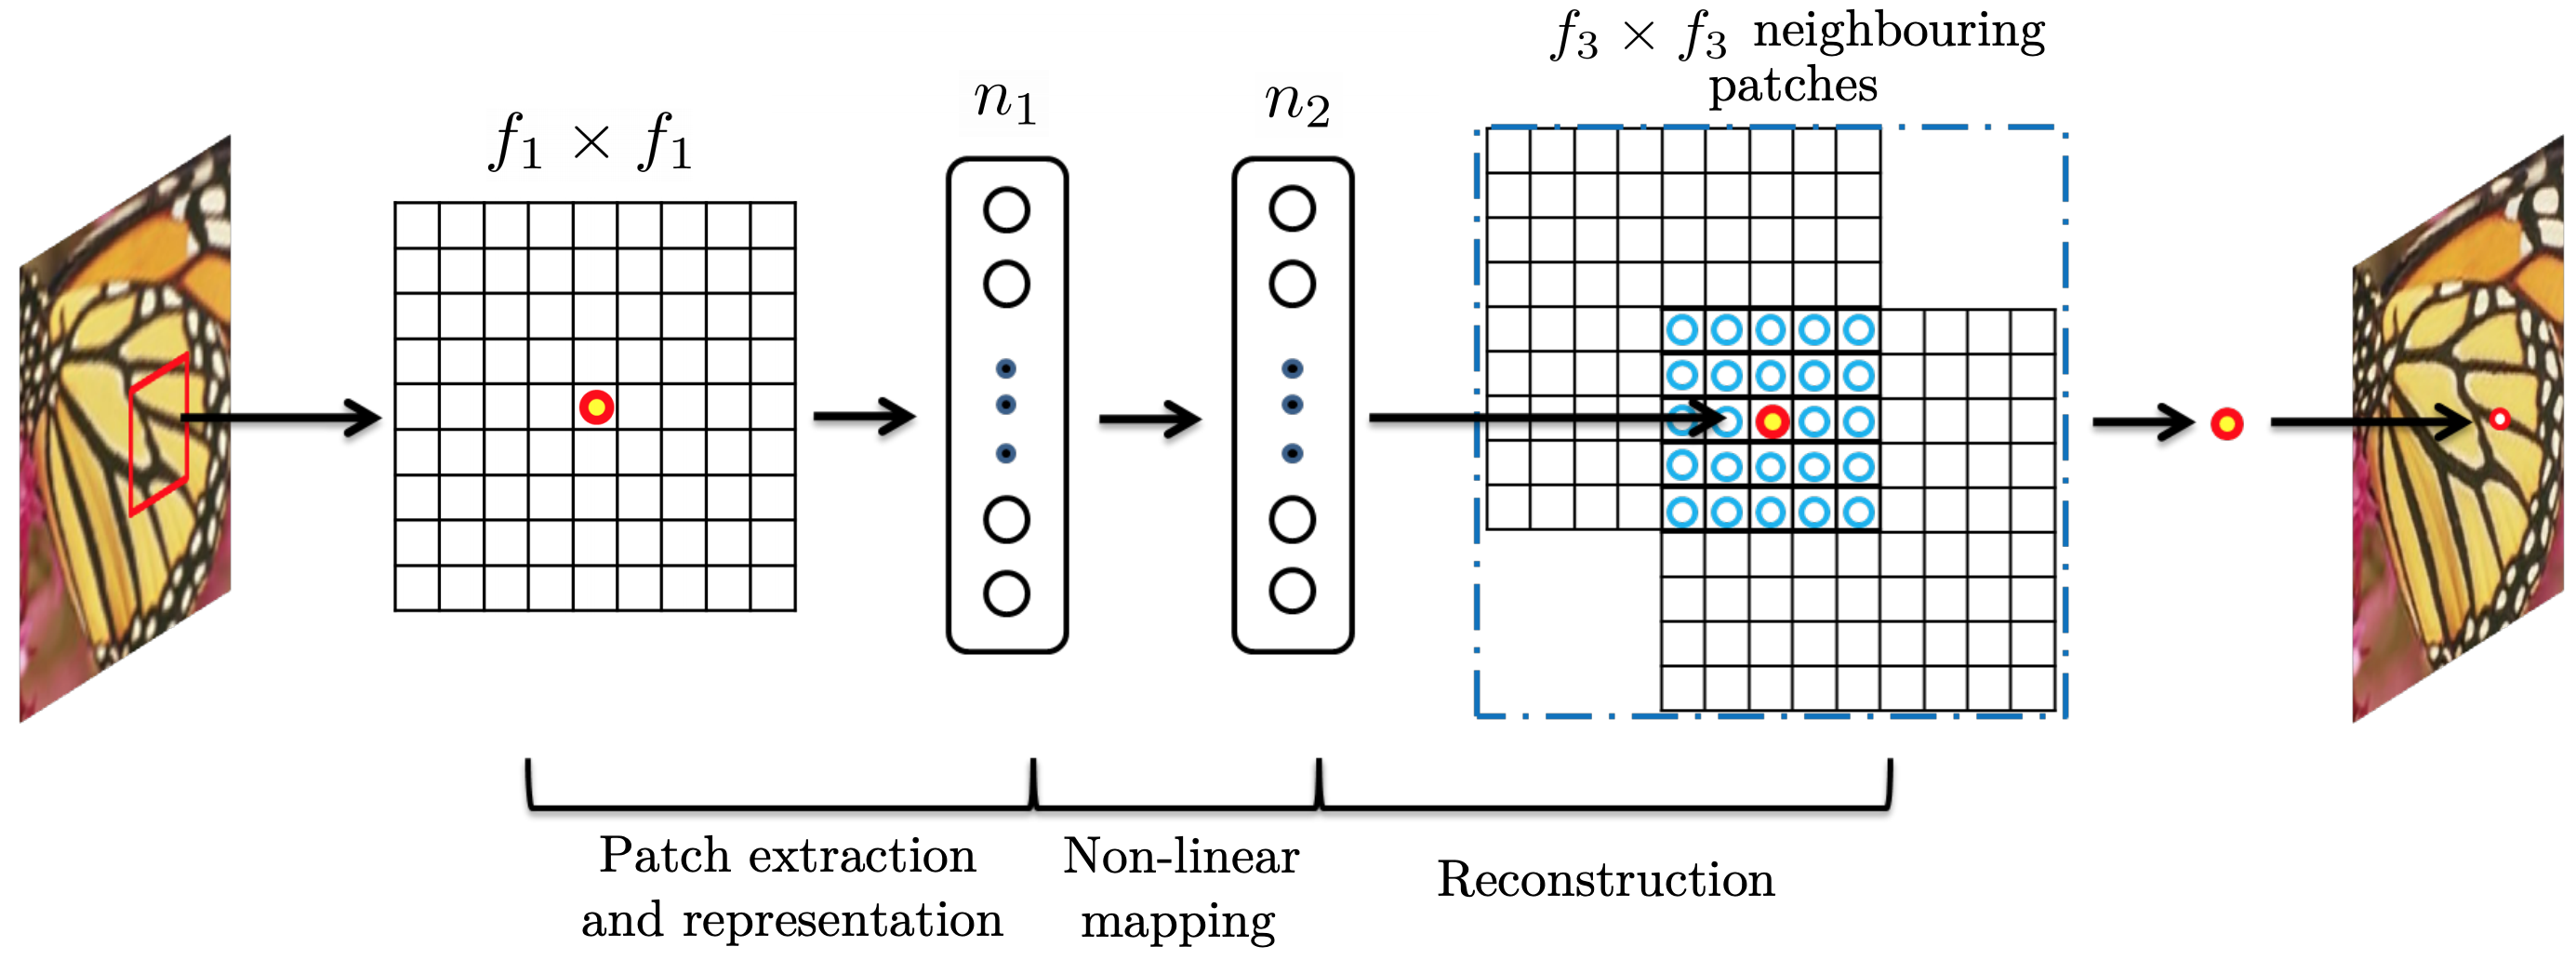
\includegraphics[width=\linewidth,keepaspectratio]{figures/neural_networks/sparse_coding.png}
        \caption{Sparse coding SR pipeline (see section~\ref{subsubsec:sparsecoding}).}\label{subfig:srcnnsparse}
    \end{subfigure}
    \vskip\baselineskip
    \begin{subfigure}[b]{\subfigwidth}
        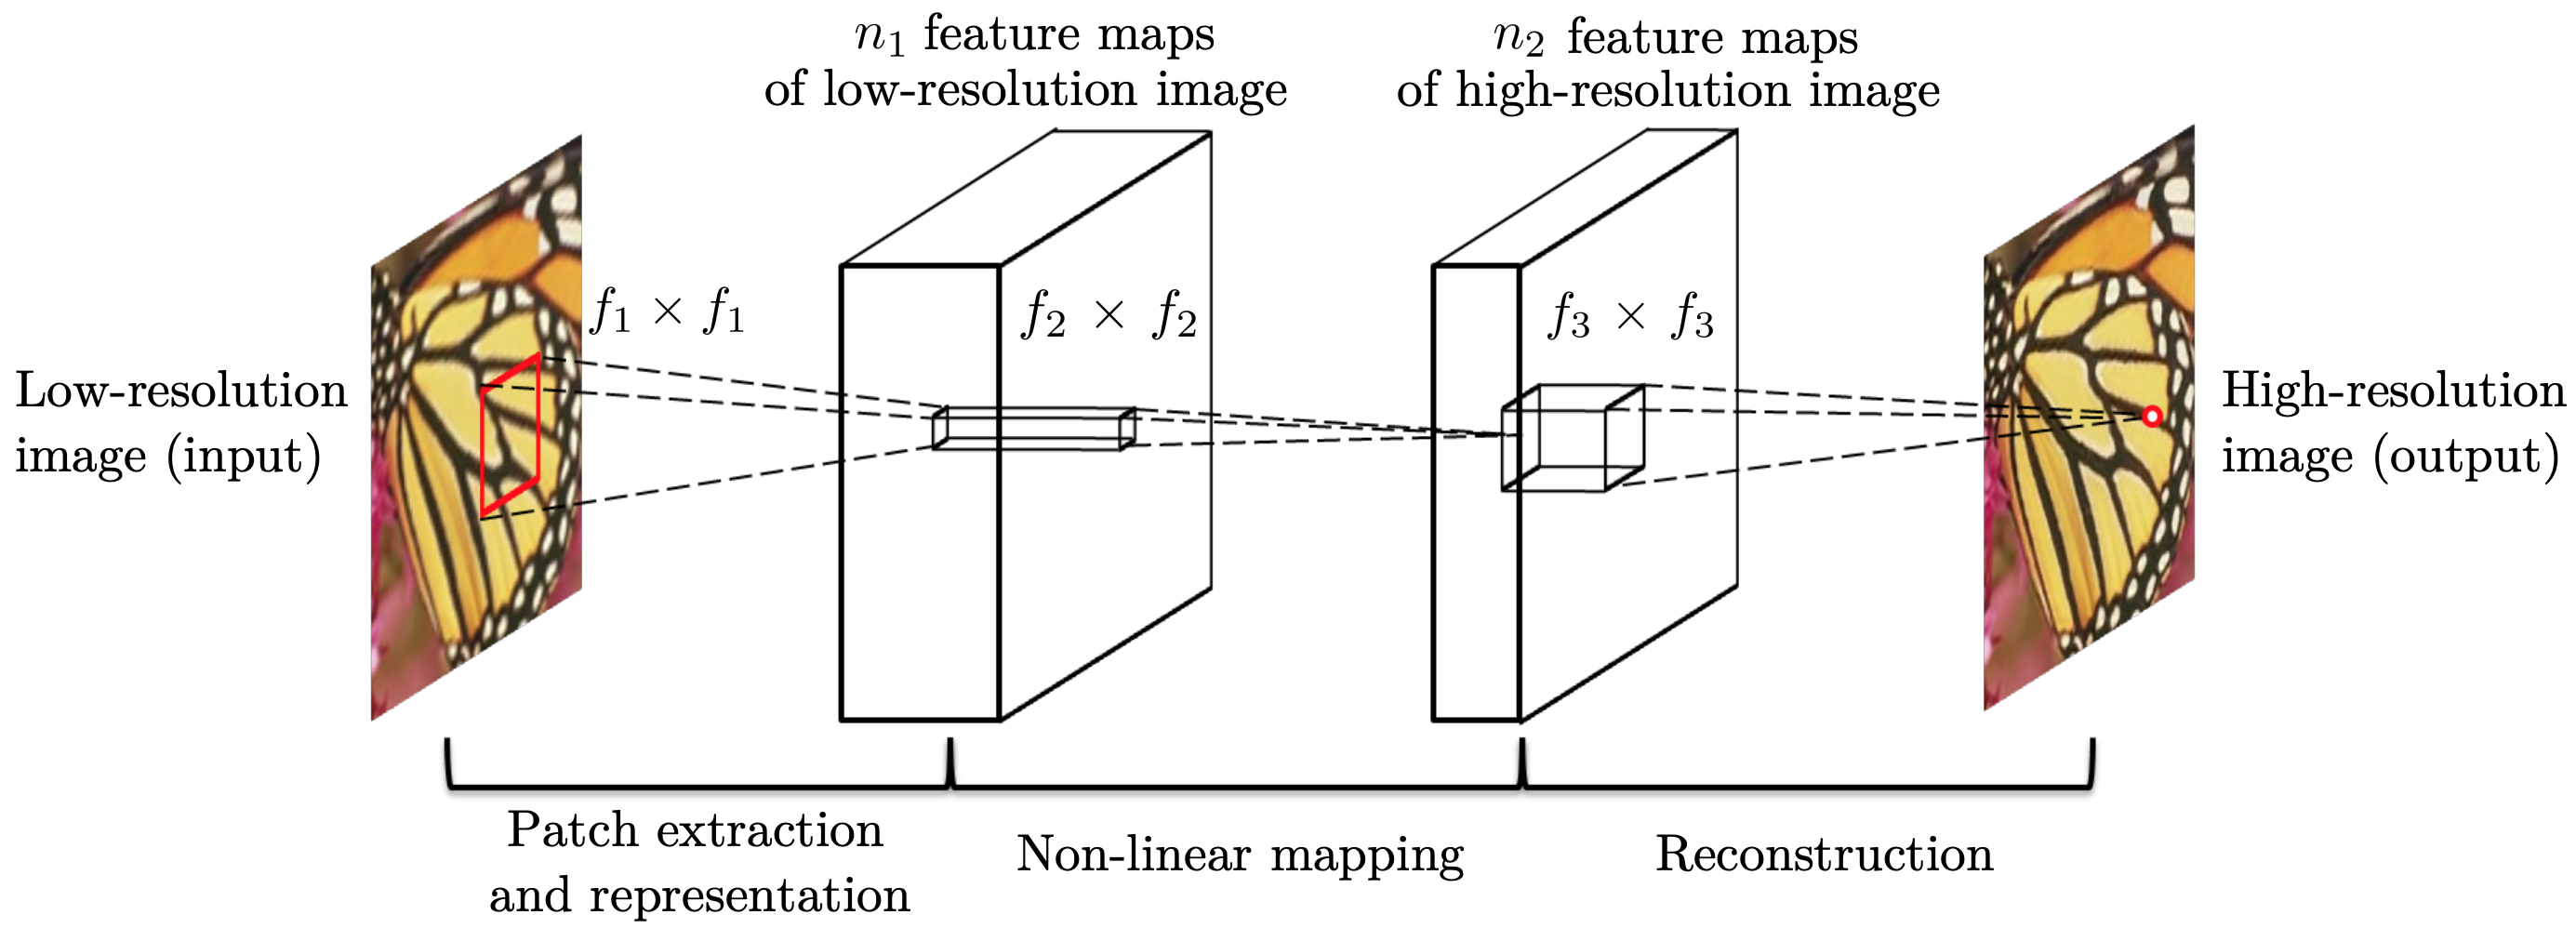
\includegraphics[width=\linewidth,keepaspectratio]{figures/neural_networks/srcnn.png}
        \caption{SRCNN pipeline.}\label{subfig:srcnn}
    \end{subfigure}
    \caption{Sparse coding SR and SRCNN comparison \cite{Dong_2016}. Note both pipelines operate on bicubic up-sampled images.}\label{fig:srcnn}
\end{figure}